\documentclass[12pt,a4paper]{amsart}
\usepackage{amsfonts}
\usepackage{amsthm}
\usepackage{amsmath}
\usepackage{amscd}
\usepackage[latin2]{inputenc}
\usepackage{t1enc}
\usepackage[mathscr]{eucal}
\usepackage{indentfirst}
\usepackage{graphicx}
\usepackage{graphics}
\usepackage{pict2e}
\usepackage{epic}
\numberwithin{equation}{section}
\usepackage[margin=2.9cm]{geometry}
\usepackage{epstopdf} 
\usepackage{appendix}
\usepackage[ruled,vlined]{algorithm2e}
\usepackage{amssymb}
\usepackage{hyperref}

 \def\numset#1{{\\mathbb #1}}

\makeatletter
\def\@tocline#1#2#3#4#5#6#7{\relax
  \ifnum #1>\c@tocdepth % then omit
  \else
    \par \addpenalty\@secpenalty\addvspace{#2}%
    \begingroup \hyphenpenalty\@M
    \@ifempty{#4}{%
      \@tempdima\csname r@tocindent\number#1\endcsname\relax
    }{%
      \@tempdima#4\relax
    }%
    \parindent\z@ \leftskip#3\relax \advance\leftskip\@tempdima\relax
    \rightskip\@pnumwidth plus4em \parfillskip-\@pnumwidth
    #5\leavevmode\hskip-\@tempdima
      \ifcase #1
       \or\or \hskip 1em \or \hskip 2em \else \hskip 3em \fi%
      #6\nobreak\relax
    \dotfill\hbox to\@pnumwidth{\@tocpagenum{#7}}\par
    \nobreak
    \endgroup
  \fi}
\makeatother
 

\theoremstyle{plain}
\newtheorem{Th}{Theorem}[section]
\newtheorem{Lemma}[Th]{Lemma}
\newtheorem{Cor}[Th]{Corollary}
\newtheorem{Prop}[Th]{Proposition}

 \theoremstyle{definition}
\newtheorem{Def}[Th]{Definition}
\newtheorem{Conj}[Th]{Conjecture}
\newtheorem{Rem}[Th]{Remark}
\newtheorem{?}[Th]{Problem}
\newtheorem{Ex}[Th]{Example}

\newcommand{\im}{\operatorname{im}}
\newcommand{\Hom}{{\rm{Hom}}}
\newcommand{\diam}{{\rm{diam}}}
\newcommand{\ovl}{\overline}
%\newcommand{\M}{\mathbb{M}}

\newcommand{\BR}{\mathbb R}
\newcommand{\BC}{\mathbb C}
\newcommand{\BE}{\mathbb E}
\newcommand{\BP}{\mathbb P}
\newcommand{\bdy}{\mathbf{y}}
\newcommand{\bdx}{\mathbf{x}}
\newcommand{\bdz}{\mathbf{z}}
\newcommand{\bdv}{\mathbf{v}}
\newcommand{\bda}{\mathbf{a}}
\newcommand{\bdb}{\mathbf{b}}
\newcommand{\bdu}{\mathbf{u}}
\newcommand{\bdw}{\mathbf{w}}
\newcommand{\bde}{\mathbf{e}}
\newcommand{\bdc}{\mathbf{c}}
\newcommand{\bdl}{\mathbf{l}}
\newcommand{\bdt}{\mathbf{t}}
\newcommand{\bdA}{\mathbf{A}}
\newcommand{\bdX}{\mathbf{X}}
\newcommand{\bdM}{\mathbf{M}}

\DeclareMathOperator{\card}{card}
\DeclareMathOperator{\argmin}{argmin}
\DeclareMathOperator{\argmax}{argmax}
\DeclareMathOperator{\supp}{supp}
\DeclareMathOperator{\Rea}{Re}
\DeclareMathOperator{\Id}{\mathbf{Id}}
\DeclareMathOperator{\var}{var}

\title{}

\begin{document}

\begin{titlepage}

\newgeometry{centering,margin=2.3in}

\begin{center}
\Large\bfseries\MakeUppercase{Lost in Sparsity: Compressed Sensing and its Applications}
\end{center}

\vskip 0.5in

\begin{center}
    \Medium\MakeUppercase{William Hartog}
\end{center}

\vskip 0.5in

\begin{center}
    \Medium{\scshape Advisors:}
    
    \Medium{\scshape Subhabrata Sen}
    
    \Medium{\scshape Clifford Taubes}
\end{center}

\vskip 2.5in

\begin{center}
    {\scshape A thesis presented in partial fulfillment of the requirements for the degree of Bachelor of Arts with Honors in Mathematics and Statistics.}
\end{center}

\vskip 0.5in

\begin{center}
    {\scshape Harvard University}
    
    {\scshape Cambridge, MA}
    
    {\scshape March 2021}
\end{center}

\end{titlepage}

\section*{Acknowledgements}

First I would like to thank my primary advisor Subhabrata Sen for being a consistently great source of knowledge and support throughout the past year, and my co-advisor Clifford Taubes for fitting reading through my thesis into his busy schedule.

I would also like to thank Patrick Lopatto, who initially recommended I look into compressed sensing for my thesis topic, and Joe Blitzstein for introducing me to statistics through three fantastically-taught courses.

Finally, I would like to thank my friends and family, especially my parents, for their love and support.

\pagebreak

\address{Harvard University \\ Departments of Mathematics and Statistics \\
Cambridge MA 02138} 

\email{whartog@college.harvard.edu}

\begin{abstract}
    The aim of this paper is to overview the history and theory of compressed sensing, a relatively new but powerful field that allows for practical and fast signal processing for signals which are sparse in some basis. We provide a geometric intuition for this requirement, as well as theoretical guarantees under which sparse recovery via $\ell^1$-minimization succeeds. We also give algorithms for the implementation of the method, a set of simulations comparing the recovery success of various algorithmic settings, and an example of applying compressed sensing to the application area of medical imaging.
\end{abstract}

\maketitle

\tableofcontents

\pagebreak

\section*{Introduction} A common mathematical and statistical problem, which is introduced in high school coursework and yet continually provides new challenges for experienced researchers, is that of solving a linear system of equations. A general setting we may consider involves a measurement matrix $\bdA\in\BC^{m\times N}$, a parameter vector or signal $\bdx\in\BC^N$, and a response vector $\bdy\in\BC^m$, satisfying
\begin{align}\label{linsys}
\bdA\bdx=\bdy.
\end{align}
For example, in the world of signal processing for image compression, which turns out to be a topic that we will very much care about, the signal $\bdx$ would be a vector comprising the parameters of the original image that we want to recover, $\bdy$ is the compressed version of this image, and$\bdA$ is a linear transformation mapping the image vector $\bdx$ to the compressed response vector $\bdy$ through the relationship (\ref{linsys}).

As such the principal problem arises when $\bdx$ is unknown but $\bdA$ and $\bdy$ are known, which boils down to an inverse problem, as is the case for the aforementioned image compression example. Such problems form the basis (pun intended) for row reduction in introductory linear algebra coursework, as well as for statistical inference in the setting of least-squares regression, where the signal $\bdx$ is interpreted as the estimated effects of a set of parameters and $\bdy$ is taken to have some error term which is usually Gaussian (alternatively known as Normal) \cite{agresti}. Moreover, this setting is exceedingly important from both mathematical and statistical perspectives because of the prevalence of this model in application, meaning solving difficult variations of the problem can often produce technologically useful results.

For methods such as these, success, as defined by the recovery of a unique exact solution or estimate for $\bdx$, can be expressed in terms of the relationship between the number of parameters, $N$, and the number of observations, $m$. Linear regression, in particular, is only a well-posed problem when the number of observations is greater than the number of solutions, and the linear system (\ref{linsys}) could possibly have a unique solution for $m\geq N$, provided certain conditions. However, the solution space $\{\bdz:\bdA\bdz=\bdy\}$ for the linear system (\ref{linsys}) will be infinite if $m<N$, meaning exact recovery of a particular $\bdx$ requires additional specifications. 

While this difficulty might appear a deterrent, a natural motivation to further investigate the $m<N$ case is that in application the ability to successfully recover signals with fewer measurements is much more practical, especially as the dimension of the parameter vector increases. Such time- and resource-saving measures have always been significant, but especially in the modern age of big data and large-scale computation, minute reductions in the number of measurements scale quickly and are instrumental to the production of cost-efficient technology. As such, the pursuit of theoretical minimums on the number of observations for such a system has been an ongoing object of scientific inquiry.

A common intuitive explanation for the ability to obtain unique solutions for systems of linear equations goes along the lines of the following adage: "As many equations as unknowns". In our context, when our parameter vector $\bdx$ has fixed length $N$, and we want to decrease the number of measurements $m$, there is no way to achieve this balance if we treat every parameter in $\bdx$ as a separate unknown. The crucial realization here is that most data follows a certain structure. For example if every row vector in the set of row vectors $\{\bdA_i\}_{i\in[m]}$ can be expressed in some set of linearly independent vectors $\{\bdb_j\}_{j\in[d]}$ that span a subspace $U\subset\BC^N$ of dimension $d<N$. Note that $[d]$ is shorthand for the set of integers $[d]:=\{1,2,...,d\}$. After adding vectors to form a basis of $\BC^N$, we can re-express the measurement matrix with this new basis, and our new parameter vector will only have nonzero entries for the first $d$ components (corresponding with our set of $d$ vectors that span $U$).

This intuitive approach nicely demonstrates how the goal of decreasing the number of measurements $m$ corresponds with the low-dimensional structure of the parameter vector, and thus sparsity of $\bdx$. Defining $\supp(\bdx):=\{i\in[N]:\bdx_i\neq0\}$ as the support set of indices $i$ for which the $i$th entry of $\bdx$ is nonzero, we call $s:=\card(\supp(\bdx))$ the \textit{sparsity} of $\bdx$ (the cardinality or size of the support of $\bdx$), and we call $\bdx$ $s$-sparse if $\card(\supp(\bdx))\leq s$. Of course, it is important to note that in practice signals will not be exactly sparse, and rather have most entries very close to zero, but exact sparsity plays an important role in both major theoretical results and in a high-level understanding of our methods.

% This following section is a fun addendum to help visualize, which I may remove at a later time. Certainly the visuals will be better if I include it in my final version

Hopefully the previous discussion is helpful to understand the importance of sparsity, but to further visualize why sparsity allows for significantly faster recovery, consider the dichotomy between two cities, represented in terms of the projection of their skylines onto a one-dimensional space. The first city, on the left of Figure \ref{ill}, is called Sparse City, and is mostly comprised of low rise buildings and a few very tall skyscrapers. A reasonable real world comparison to Sparse City is Los Angeles, which has much fewer skyscrapers than other, shorter buildings. On the other end of the spectrum is Dense City, on the right of Figure \ref{ill}, in which practically every building is of a sizable height, including many larger skyscrapers. Dense City can be compared to New York City, which is known for its very dense skyline of large buildings.


\begin{figure}
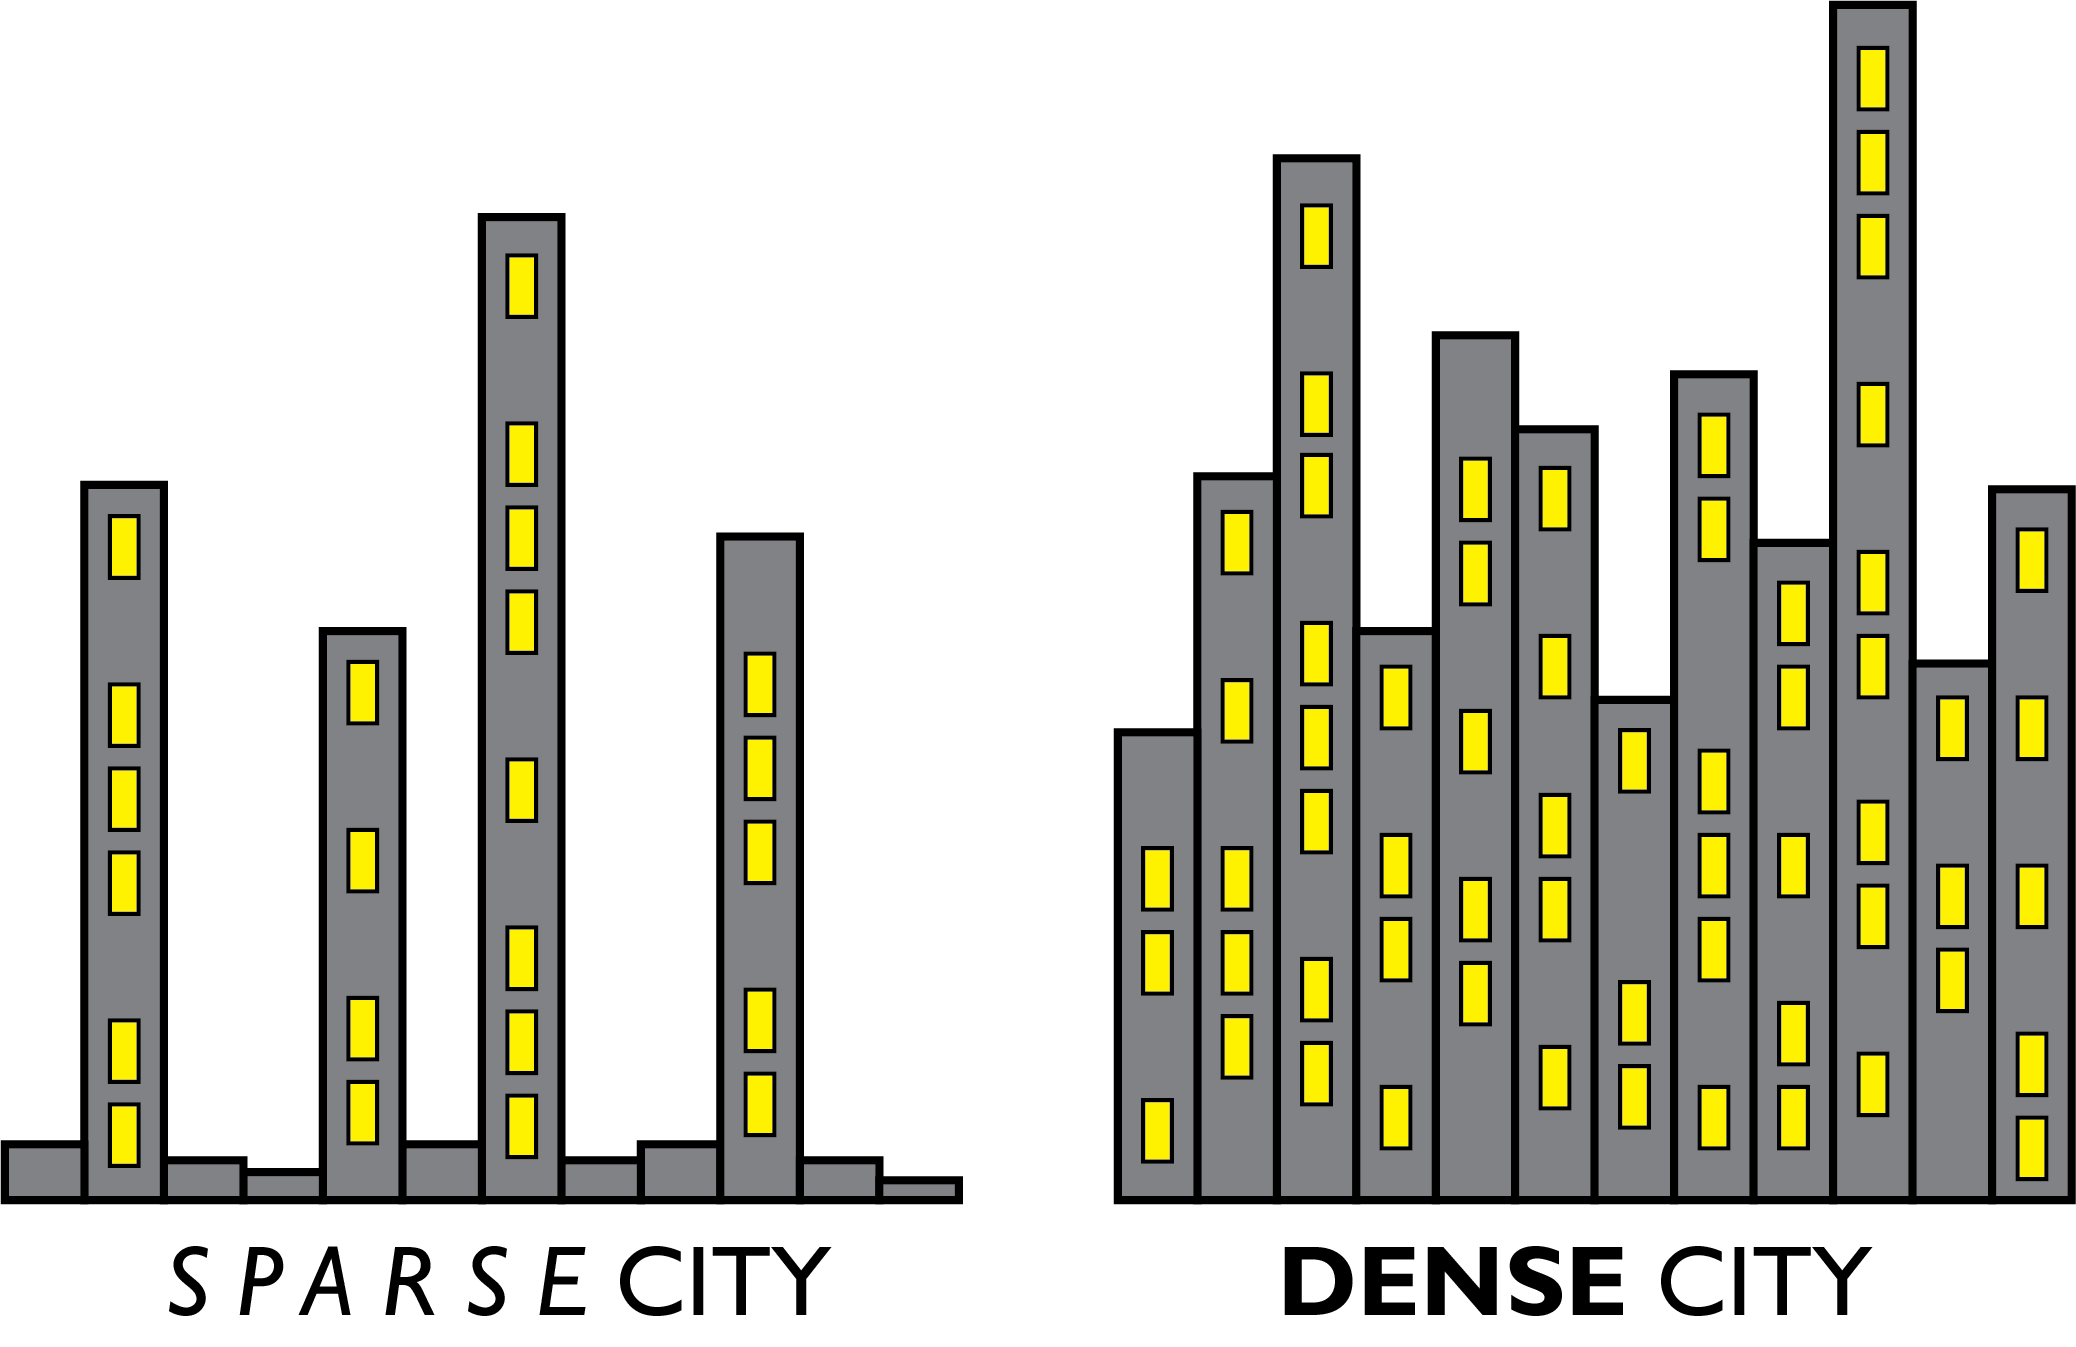
\includegraphics[scale = 0.7]{sparse_dense_city_final.png}
\caption{Illustration depicting the hypothetical Sparse City and Dense City, whose differences are characterized by the number of buildings with non-negligible heights.}
\label{ill}
\end{figure}

If asked to exactly reconstruct the heights and locations of all "sizable" buildings in Sparse City and Dense City, it clearly seems doing so for Sparse City would be the easier task, in the sense that less information would be required. To draw a comparison to our linear system setting, we need a notion of what a "measurement" is, but any way you might take a measurement, including taking various snapshots of the city, the sparse nature and clear structure of Sparse City make it the easier of the two cities to classify.

% here ends the addendum section

\subsection*{The History of Signal Processing and Sampling Theorems}

Armed with a specific target of sparsity through low-dimensional structures in our experiments, we turn to what has historically been a rich pursuit of low-dimensional structures in statistical inquiry.

One reason low-dimensional structures have been a common point of academic interest is a hypothesis that human natural vision is an example of sparse recovery \cite{wm}. Natural vision systems are able to display highly accurate representations of their perceived reality incredibly well, in terms of time and efficiency. In particular, potential measurements contain a high amount of extraneous information, and thus a primary purpose of natural vision is to recreate these images while minimizing redundancy in observation. 

This natural example of exploitation of low-dimensional structures motivates the investigation by engineers into image processing using computers through a similar exploitation \cite{wm}. Of course images hardly represent of the spectrum of real-world data that are sparse in some way, as we see in the history of low-dimensional structures in statistics. 

In particular, much of this history is concerned with signals $x(t)$ that are functions of time $t$ and often represent data such as audio signals. Then we will look at the set of signals that are "band-limited", which are formally defined as functions such that their Fourier transform
\begin{align*}
    \hat x(\omega)=\int_{-\infty}^\infty x(t)\exp(-i\omega t)dt
\end{align*}
vanishes for $\omega$ outside of some interval $[-\Omega,\Omega]$, which translates to the condition that a signal has a maximum frequency of $f_{\max}=\Omega/2\pi$. This may appear an improper structure to investigate if we cared about a discrete signal such as an image with finitely many pixels. However the results on recovery of such signals via sampling are rich when taking finitely many measurements of a signal, for example by taking measurements $x(\frac{n\pi}{2})$ for integers $n$, where $\{\frac{n\pi}{2}\}_n$ are the associated time values. We call $\mathcal{B}_1(\Omega)$ the set of band-limited functions with associated constant $\Omega$.

A characterization of the minimum number of samples required for band-limited signal recovery given in the 1920s is attributed to Harry Nyquist and Claude Shannon (though earlier proposed by E.T. Whittaker in 1915 and later by Vladimir Kotelnikov) \cite{wm}:

\begin{Th}{(Nyquist-Shannon Sampling)}\label{n-s}  To recover a band-limited signal $x(t)$ with $x\in\mathcal{B}_1(\Omega)$, it is necessary to sample the signal at a rate twice the maximum frequency $f_{\max}=\Omega/2\pi$.

\end{Th}

We omit the proof of this theorem, but note that while powerful, it can become rather inefficient, especially when the maximum frequency becomes rather large while the range of frequencies stays the same. Intuitively we would like to obtain the same sampling rate for a given frequency range, regardless of its location in the spectrum \cite{wm}. Sampling at what is usually known as the Nyquist sampling rate is costly, and can be potentially dangerous for patients in medical imaging, so an alternative approach would be welcome. This is not at all to understate the value and impact of the Nyquist sampling scheme, which was so commonly used in signal processing that a major improvement on the Nyquist rate was sure to be a landmark result.

\subsection*{The Failure of $\ell^0$-Minimization and the Embrace of $\ell^1$-Minimization}

A natural way to approach the problem of sparse recovery is as a minimization problem with respect to the $\ell^0$ norm. The $\ell^0$ norm of $\bdx$, $\|\bdx\|_0=|\supp(\bdx)|$, which is the number of nonzero entries in the vector $\bdx$, is just the sparsity of $\bdx$ as we defined earlier. This gives rise to the optimization problem known as $\ell^0$-minimization.
\begin{align} \label{l0}
    \text{minimize } \|\bdz\|_0 \ \ \ \ \text{subject to } \bdA\bdz=\bdy.
\end{align}
However, $\ell^0$-minimization is known to be an NP-hard problem in the worst case \cite{fou-rau}, which doesn't bode well for its utility. Specifically, the problem, when generalized to the condition that $\|\bdA\bdz-\bdy\|_2\leq\eta$ (where $\|\cdot\|_2$ is the $\ell^2$ norm defined as $\|\bdz\|_2=\sqrt{\sum_{i=1}^m|\bdz|_i^2}$ for $\bdz\in\BR^m$) for some fixed $\eta\geq0$, is NP-hard, which is proven in \cite{fou-rau} via reduction to the exact cover problem with 3-sets, a brief description of which is as follows:

\begin{Def}\label{exact-cover} The \textbf{Exact Cover by 3-Sets Problem} is to find, for some collection of sets $C=\{\mathcal{C}_i\}_{i\in[N]}$ with $\mathcal{C}_i\subset[m]$ and $|\mathcal{C}_i|=3$ for all $i\in[N]$, a partition of $[m]$ using elements of $C$, i.e. some index set $J\subset[N]$ with $\{\mathcal{C}_j\}_{j\in J}$ disjoint and $\cup_{j\in J}\mathcal{C}_j=[m]$.
\end{Def}

We omit the proof of this reduction, which can be found in \cite{fou-rau}.

Of course, the notion of NP-hardness is a worst case statement, and the worst case might turn out to be very rare. Nevertheless, knowledge of this worst case scenario and the persisting difficulty of exact computation for the $\ell^0$ norm \cite{haz-maz} make a case for looking for alternatives.

We might instead minimize the $\ell^1$, defined as $\|\bdx\|_1=\sum_{i=1}^N|\bdx|_i$, which would produce an output that has a small total sum of absolute entries, which is not as suitable as the $\ell^0$ norm but will turn out to be a sufficient proxy. Thus, while $\ell^0$-minimization is a natural consideration, it is not feasible as a method, either in theory or in practice, and as such we will focus our attention on the looser but more implementable $\ell^1$-minimization, which as we will see has enjoyed historical successes \cite{fou-rau, wm}.

Apart from the Nyquist rate, band-limited signals played a large role in signal recovery results in the PhD work of Benjamin Logan in the 1960s, which produced the following result regarding $\ell^1$-minimization \cite{logan}:

\begin{quote}
    Suppose we observe a signal $y$ which consists of a band-limited signal $x_0$, superimposed with an error $e_0$ which is sparse in the time domain. If the product of the bandwith of $x_0$ and the size of the support of $e_0$ is less than $\pi/2$, the true band-limited signal can be recovered by $\ell^1$ minimization, no matter how large the error is in magnitude, or where its support is located.
\end{quote}

This result, often known as Logan's Phenomenon, characterizes the ability of the method known as $\ell^1$-minimization to recover signals, where $\ell^1$-minimization in the context of Logan's work is the optimization problem
\begin{align*}
    \text{minimize } \|x-y\|_1 \ \ \ \ \text{subject to } x\in\mathcal{B}_1(\Omega),
\end{align*}

where the observed signals $y$ are obtained from the original signal $x_0$ by some offset error $y=x_0+e_0$, where $e_0$ is "sparse in the time domain" in the sense that its support is a set of small measure (which is a rigorous generalization of the geometric concept of area). Here $e_0$ is interpreted as a function $e_0:\BR\rightarrow\BR$ with input of time $t$. We refer the reader to \cite{logan} for a more complete description of the result.

Since the signals $x$ are continuous functions, we interpret $\|\cdot\|_1$ the $\ell^1$ norm differently than on $\BC^n$, but Logan's Phenomenon marks a first example of the usefulness of $\ell^1$-minimization as an approach for successfully recovering sparse signals, with more examples to follow in the latter decades of the 20th century \cite{wm}. With regard to our main environment of interest, when we want to recover $\bdx\in\BC^N$ given the measurement $\bdy=\bdA\bdx$ where $\bdy\in\BC^m$ and $\bdA\in\BC^{m\times N}$, lasso regression is a particularly popular algorithm, which is formulated as follows (with $\|\cdot\|_2$ the $\ell^2$ norm as defined earlier in the section):
\begin{align*}
    \text{minimize}_\bdz\text{ } \|\bdy-\bdA\bdz\|_2^2 \ \ \ \ \text{subject to } \|\bdz\|_1\leq k.
\end{align*}
In fact, lasso is equivalent in formulation to basis pursuit, which is another optimization based on the $\ell^1$ norm \cite{wm}:
\begin{align} \label{l1}
    \text{minimize } \|\bdz\|_1 \ \ \ \ \text{subject to } \bdA\bdz=\bdy.
\end{align}
Given this clear objective, which is to achieve a more efficient sampling rate than the standard Nyquist rate, and a useful tool, $\ell^1$-minimization (intuition for which we will further develop in Section \ref{geom-int}), the ground is set for a major breakthrough.

\subsection*{Compressed Sensing: The Seminal Work}

With this backdrop of $\ell^1$ norm methods for signal recovery from the latter half of the 20th century, the ball was bound to drop, in the eye of what John Wright and Yi Ma describe as a "perfect storm" \cite{wm}. Between 2005 and 2006, through a collaboration betweenEmmanuel Cand\`{e}s, Justin Romberg, Terence Tao, and David Donoho \cite{candes, donoho}, the observation that $\ell^1$-minimization performed recovery of sparse signals with few measurements was formalized into what became known as the field of compressed sensing (CS), and can alternatively be known by any combination of $\{\text{compressed, compressive}\}$ and $\{\text{sensing, sampling}\}$ \cite{fou-rau,wm}. Their key results were the ability to recover a sparse signal $\bdx\in\BC^N$ supported on a set of size proportional to $N$, with a number of measurements $m$ that significantly bests the Nyquist rate, through a random measurement matrix $\bdA\in\BC^{m\times N}$. 

Precise statements of such results are given in Section \ref{theory}. In addition, the usage of a random measurement matrix is a crucial development, which we will likewise expound on in later sections. The importance of the work of these academics, and the further development of general results in Cand\`{e}s and Tao's 2006 paper "\textit{Decoding by Linear Programming}" contributed to a veritable explosion of work in the budding field of compressed sensing. By 2010 additional theoretical and applied results were produced on the subject, including multiple applications of the method to industry, including most notably medical resonance imaging (MRI) and the single-pixel camera, but also radar technology, sparse approximation, machine learning, and facial recognition \cite{fou-rau, wm}. Since this initial boom, compressed sensing has proven to be a valuable numerical method, especially in the age of big data.

As such, this paper covers three main topics as relating to the field of compressed sensing. First, we provide an overview of the theory behind compressed sensing, namely the method of $\ell^1$-minimization, the conditions under which $\ell^1$-minimization succeeds at sparse recovery, and the need for random matrices (Sections \ref{geom-int} and \ref{theory}). Second, we highlight a few of the more commonly used algorithms for implementing compressed sensing, including a comparison of their performances on simulated datasets (Section \ref{algs}). Third, we give an example of what an application of compressed sensing looks like in practice, in the field of MRI, since the power of the field lies in its applicability, and most of the current challenges in compressed sensing involve its application to real data (Section \ref{app}).

\section{Geometric Intuition for $\ell^1$-Minimization}\label{geom-int}

As mentioned in the Introduction, compressed sensing relies on an optimization method that had been in use for years before the seminal work of Donoho, Cand\`{e}s, Romberg, and Tao, $\ell^1$-minimization (\ref{l1}). While the historical success of this method may assuage potential concerns, it remains that the accuracy of $\ell^1$-minimization in sparse recovery is not as clear as that of $\ell^0$-minimization (\ref{l0}). Specifically, minimizing the $\ell^1$ norm $\|\bdx\|_1$ at face value does not produce sparse vectors as outputs, while the whole point of compressed sensing is to like to recover vectors which are sparse.

For this reason we take a brief aside into the geometry of the $\ell^1$ norm and why the problem as constructed is well-formulated. 

With regard to the minimization problem (\ref{l1}), we know the solution space is
\begin{align*}
    \{\bdx\}+\ker(\bdA)=\{\bdx+\bdu:\bdu\in\ker(\bdA)\}
\end{align*}
where the kernel is defined as the set $\ker(\bdA)=\{\bdu\in\BC^N:\bdA\bdu=0\}$. In all of these cases $\ker(\bdA)$ is a hyperplane in $\BC^N$, where we wish to find the point $\bdz\in S$ on that hyperplane which minimizes its $\ell^1$ norm $\|\bdz\|_1$. Using a graphical representation adapted from Wright and Ma \cite{wm} we can represent this problem in the case of domain $\BR^3$ for simplicity, which we show in Figure \ref{R3-ball}. Here, we can think of starting with the unit $\ell^1$ ball (or some scaled down version such that it does not intersect the feasible set $\{\bdx\}+\ker(\bdA)$), which appears as a diamond in $\BR^3$, and subsequently increasing the radius of the ball until it first intersects the feasible set. That first intersection point will subsequently be the output of an $\ell^1$-minimization algorithm, since all other points with smaller $\ell^1$ norm (namely the points in the earlier $\ell^1$ balls) were separated from the hyperplane $\{\bdx\}+\ker(\bdA)$. It is apparent that this minimizer might not in general be unique, as if for example the solution space is parallel with the closest face of the $\ell^1$ ball then there would be multiple solutions.

An important visualization to associate with this minimization is that the $\ell^1$ ball is convex, as for $x,y\in B_1$, and $t\in[0,1]$, we get that
\begin{align*}
    \|tx+(1-t)y\|_1\leq t\|x\|_1+(1-t)\|y\|_1\leq t+1-t=1,
\end{align*} so $tx+(1-t)y\in B_1$ as well. In addition, its image under a linear map (such as $\bdA$ in Figure \ref{polytope}) is likewise convex. In particular this convexity is geometrically sharp rather than smooth. As seen in Figure \ref{R3-ball}, the unit ball in $\BR^3$ is a diamond-like solid, with flat faces, and sharp edges and vertices.

\begin{figure}
    \centering
    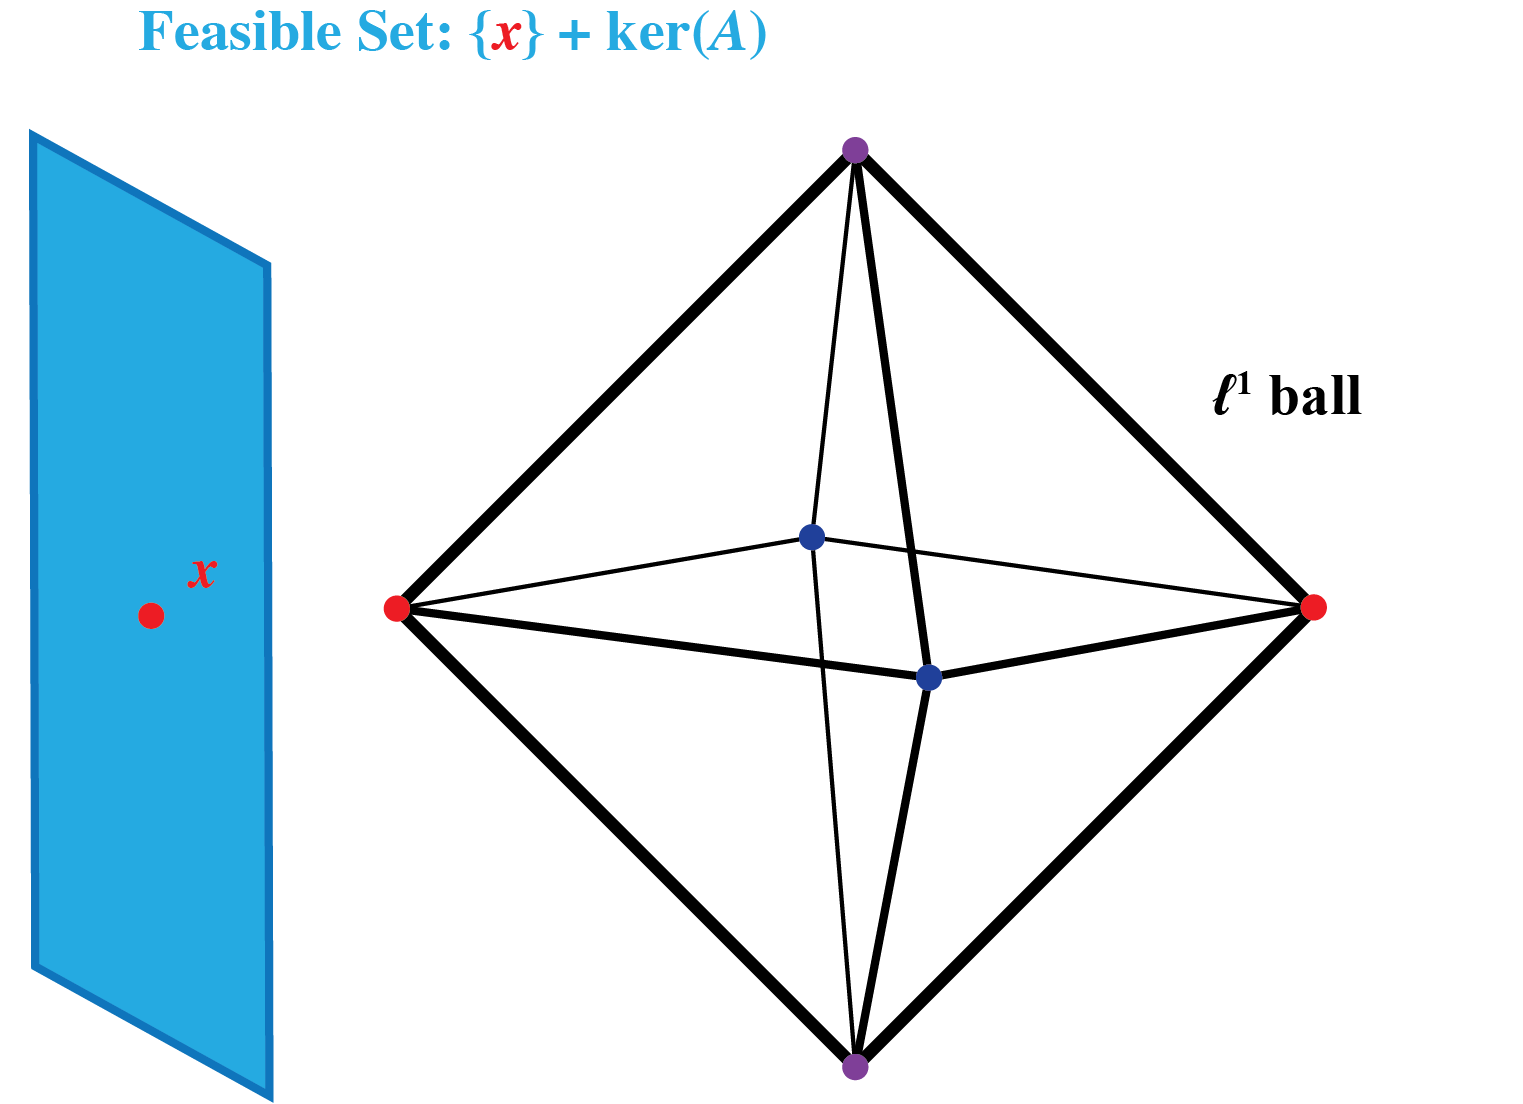
\includegraphics[scale = 0.7]{l1ball_illustration_final.png}
    \caption{Visualization of the $\ell^1$ ball in $\BR^3$ ($B_1$) and a feasible set of solutions $\{\bdz:\bdA\bdz=\bdA\bdx\}$. Performing $\ell^1$-minimization consists of scaling the $\ell^1$ ball by $t$ and taking the first point of intersection of the feasible set with $tB_1$. Because of the jagged nature of $B_1$ this will most likely be a sparse vector. This diagram is based on a figure from Wright and Ma \cite{wm}.}
    \label{R3-ball}
\end{figure}

Unfortunately, it is not straightforward to generalize this low-dimensional case to the large value of $N$ which we hope to work with in compressed sensing. However, it provides an excellent visualization of a fortunate result, which is that the first intersection point will with high probability be at one of the corners of the $\ell^1$ ball, which are precisely the vectors $\bdz\in\BR^3$ with only one nonzero entry (i.e. those that are 1-sparse).

We may also visualize a similar and related process in the target space, generally $\BC^m$, with the images of $\bdx$ and the $\ell^1$ ball $B_1$. Again adapted from Wright and Ma \cite{wm}, in Figure \ref{polytope} we represent the recovery process as expanding the image of the $\ell^1$ ball in $\BC^m$ until it hits $\bdA\bdx$, where for some $t\in\BR$, $\bdA\bdx\in\partial(t\bdA(B_1))$. Here $\partial(t\bdA(B_1))$ is the boundary of the image of the $\ell^1$ ball scaled by $t$. Note that Figure \ref{R3-ball} and \ref{polytope} differ in that the feasible set in Figure \ref{R3-ball} is visualized by a matrix $\bdA$ with two-dimensional kernel (thereby producing a plane in $\BR^3$, while we do not necessarily have the same restriction on $\bdA$ for Figure \ref{polytope}.

The key takeaway here is that recovery will be successful if the $\ell^1$ normalized version of $\bdx$, $\frac{\bdx}{\|\bdx\|_1}\in B_1$, gets mapped under $\bdA$ to the outside of the convex polytope $\bdA(B_1)$, so if $\bdA\frac{\bdx}{\|\bdx\|_1}\in\partial(\bdA B_1)$. In particular, note that in this example while the vertices of the convex polytope are the images of the vertices of the unit ball $B_1$ (which in turn are the 1-sparse vectors with only one nonzero entry). As we increase sparsity, and look at the images of the edges of $B_1$ (which are the 2-sparse vectors with two nonzero entries), we see that some, though not all, of these edges get mapped to the outside of the polytope, which is visualized by the line segments in the interior of the polytope. Thus, at least for this 3-dimensional case, once we get past the 1-sparse level, recovery is not guaranteed.

\begin{figure}
    \centering
    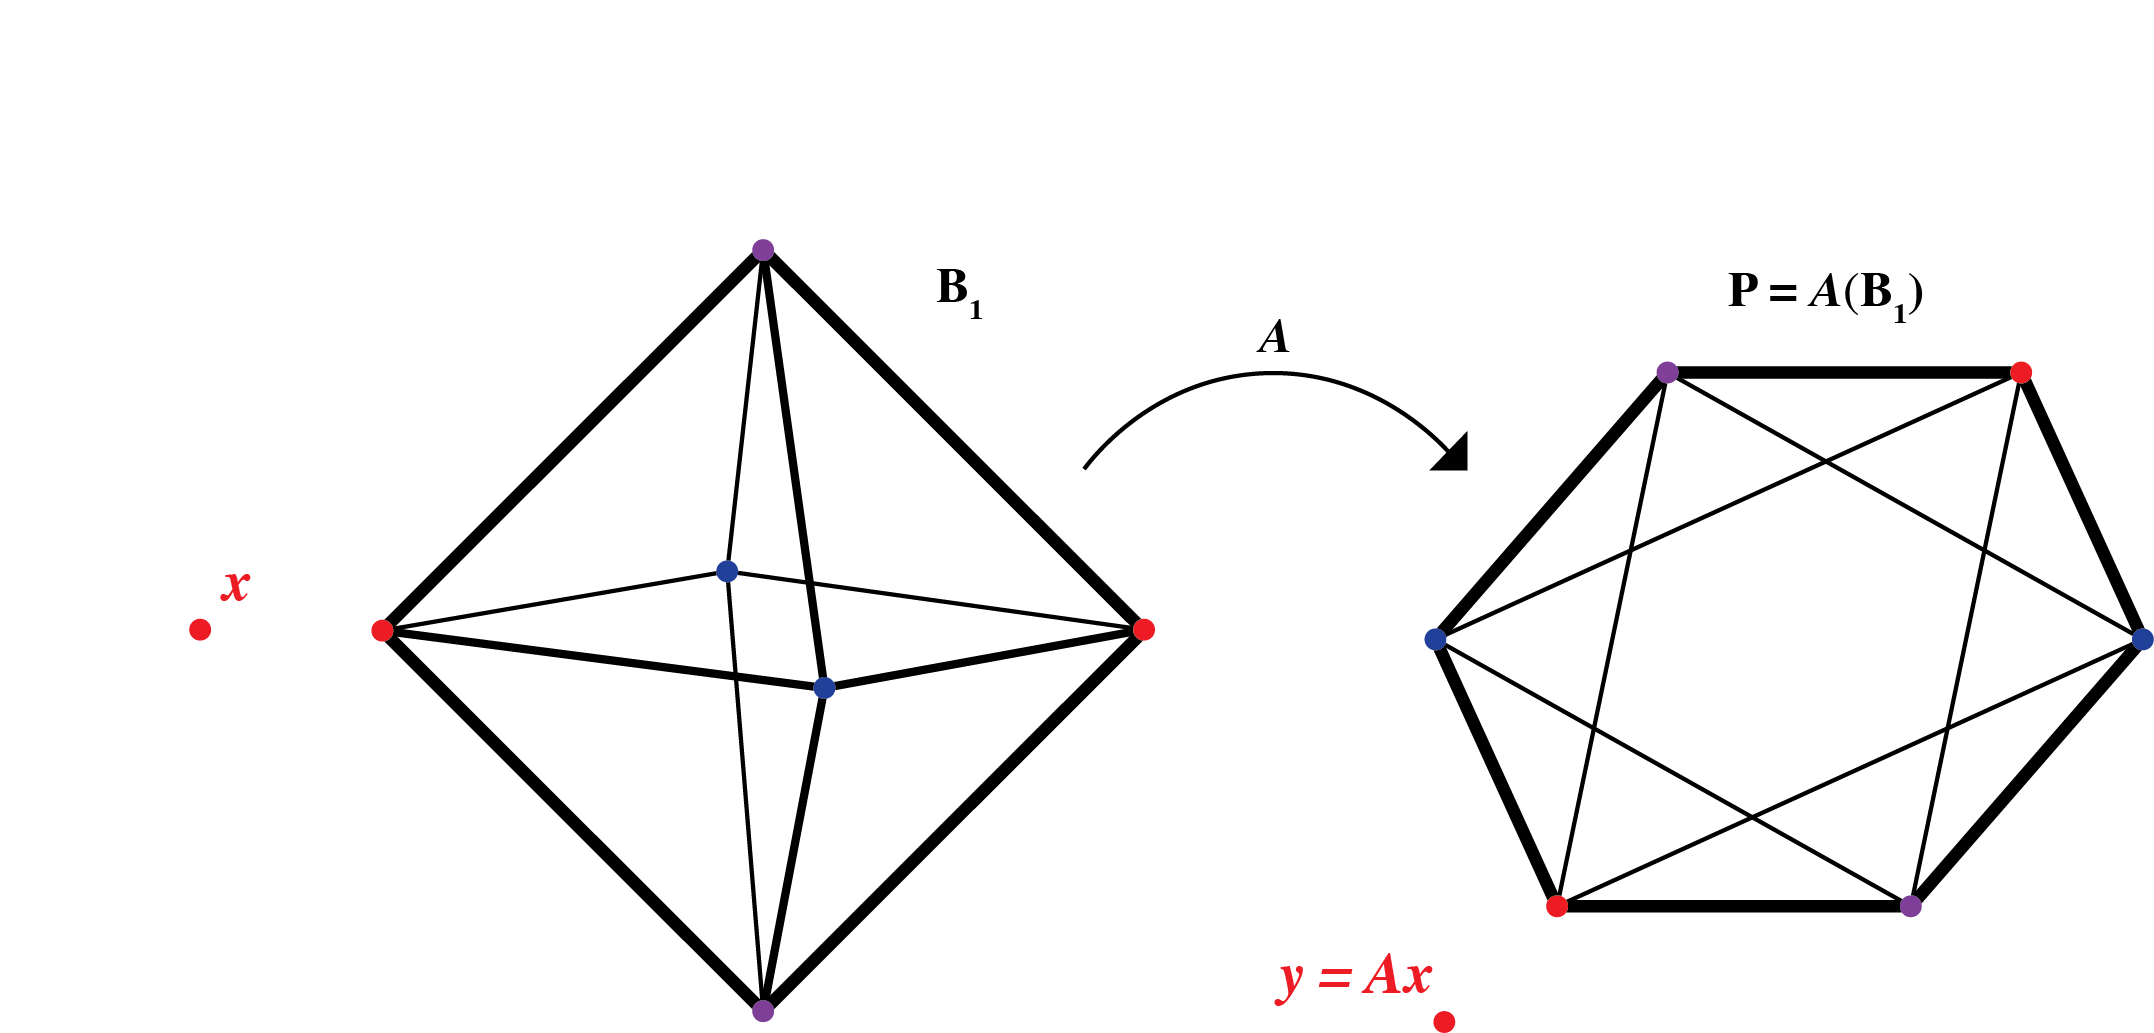
\includegraphics[scale = 0.7]{l1ball_transform_final.png}
    \caption{Visualization of a possible mapping of the $\ell^1$ ball $B_1$ in $\BR^3$ to the convex polytope $P=\bdA(B_1)$ in $\BR^2$. If we scale the sets by $t$, the first point of intersection of $\bdy$ and $t\bdA(B_1)$ will correspond to the output of $\ell^1$-minimization. This diagram is based on a figure from Wright and Ma \cite{wm}.}
    \label{polytope}
\end{figure}

However, when extending this picture to higher dimensions, we will find it actually becomes easier for $\ell^1$-minimization to recover signals as the target space and associated convex polytope grow in dimension. For particular choices of $\bdA$ (an understanding of which choice we will spend Section \ref{theory} exploring), the multi-dimensional faces of the boundary of $\bdA(B_1)$ will represent the images of signals with a suitably high sparsity, which we will also formalize soon. 

In addition, the volume of the $\ell^1$ ball $B_1^N:=\{\bdx\in\BR^N:\|\bdx\|_1\leq1\}$ will approach zero as $N\rightarrow\infty$, which helps to intuitively understand why sparse recover will grow easier as $N$ increases. While we cannot visualize this progression, the best proxy is to think of the ball as becoming progressively more spiky, with the spiky parts corresponding to sparse vectors, which naturally entails easier signal recovery for such sparse signals.

In particular, the ratio of the volumes of the $\ell^1$ unit ball $B_1^N$ to the $\ell^2$ unit ball $B_2^N:=\{\bdx\in\B^N:\|\bdx\|_2\leq1\}$, using formulas for their volumes found in \cite{wang}, will approach 0 as $N\rightarrow\infty$. Furthermore, if one inscribed a Euclidean ball inside $B_1^N$, the $\ell^1$ ball of dimension $N$, the volume of that Euclidean ball would converge to 0 as $N\rightarrow\infty$ \cite{vershynin}. This latter point can be interpreted as showing that the central part of $B_1^N$ becomes very small, with most of its volume present at the tips, hence the notion of a spiky geometry, though we are unable to literally visualize the ball in higher dimensions.

These observations provide for us a much better picture of why $\ell^1$-minimization is in fact a worthy substitute for $\ell^0$-minimization, and as such we are ready to develop an understanding of how to choose cooperative measurement matrices $\bdA$ to pair with this method.

\section{Theoretical Guarantees for Successful Recovery}\label{theory}

This is where the fun begins. In this section we introduce results, usually of the following form: "If the measurement matrix $\bdA\in\BC^{m\times N}$ behaves the following regularity property, then $\bdx\in\BC^N$ is the unique solution to the optimization problem (\ref{l1})". Continuing the trend established in Section \ref{geom-int}, we will often justify these regularity properties through a geometric interpretation. Two such results involve the coherence and restricted isometry constants of a matrix, which are developed in Sections \ref{coh-section} and \ref{rip-section}, and Sections \ref{random-matrix} and \ref{gaussian-pf} detail why random matrices are necessary to satisfy the restricted isometry property, a recovery condition based on the restricted isometry constant.

\subsection{Coherence}\label{coh-section}

First we introduce coherence, a measure associated with a given matrix $\bdA$ which gives a sense of the linear dependence between the columns of $\bdA$. In particular, it is easiest to recover a sparse vector supported on $S\subset[N]$ when we know that the columns of $\bdA$ on that index set are nearly mutually orthogonal, or intuitively, when the columns are more distinguishable from each other. The coherence measure gives a value corresponding to the worst case for any index set of size $s$, so the lower the coherence, the more easily we would expect to achieve sparse recovery. First we define the general coherence function $\mu$ (with implicit argument $\bda\in\BC^{m\times N}$ where $\bda_i\in\BC^m$ is the $i$th column vector of $\bdA$)
\begin{align}
    \mu:=\max_{1\leq i\neq j\leq N}|\langle\bda_i,\bda_j\rangle|,
\end{align}

which is the worst case scenario for the dependence between any two of the column vectors. Note that $\langle\cdot,\cdot\rangle$ is the standard inner product for $\BC^m$, so $|\langle\bda_i,\bda_j\rangle|$ is interpreted geometrically as the dependence between the two column vectors. A quick visualization in two dimensions of what constitutes a more incoherent set of vectors is given in Figure \ref{coh-vis}, noting that as the dimensionality $m$ of the column vectors increases, it becomes easier to space out many vectors evenly.

\begin{figure}
    \centering
    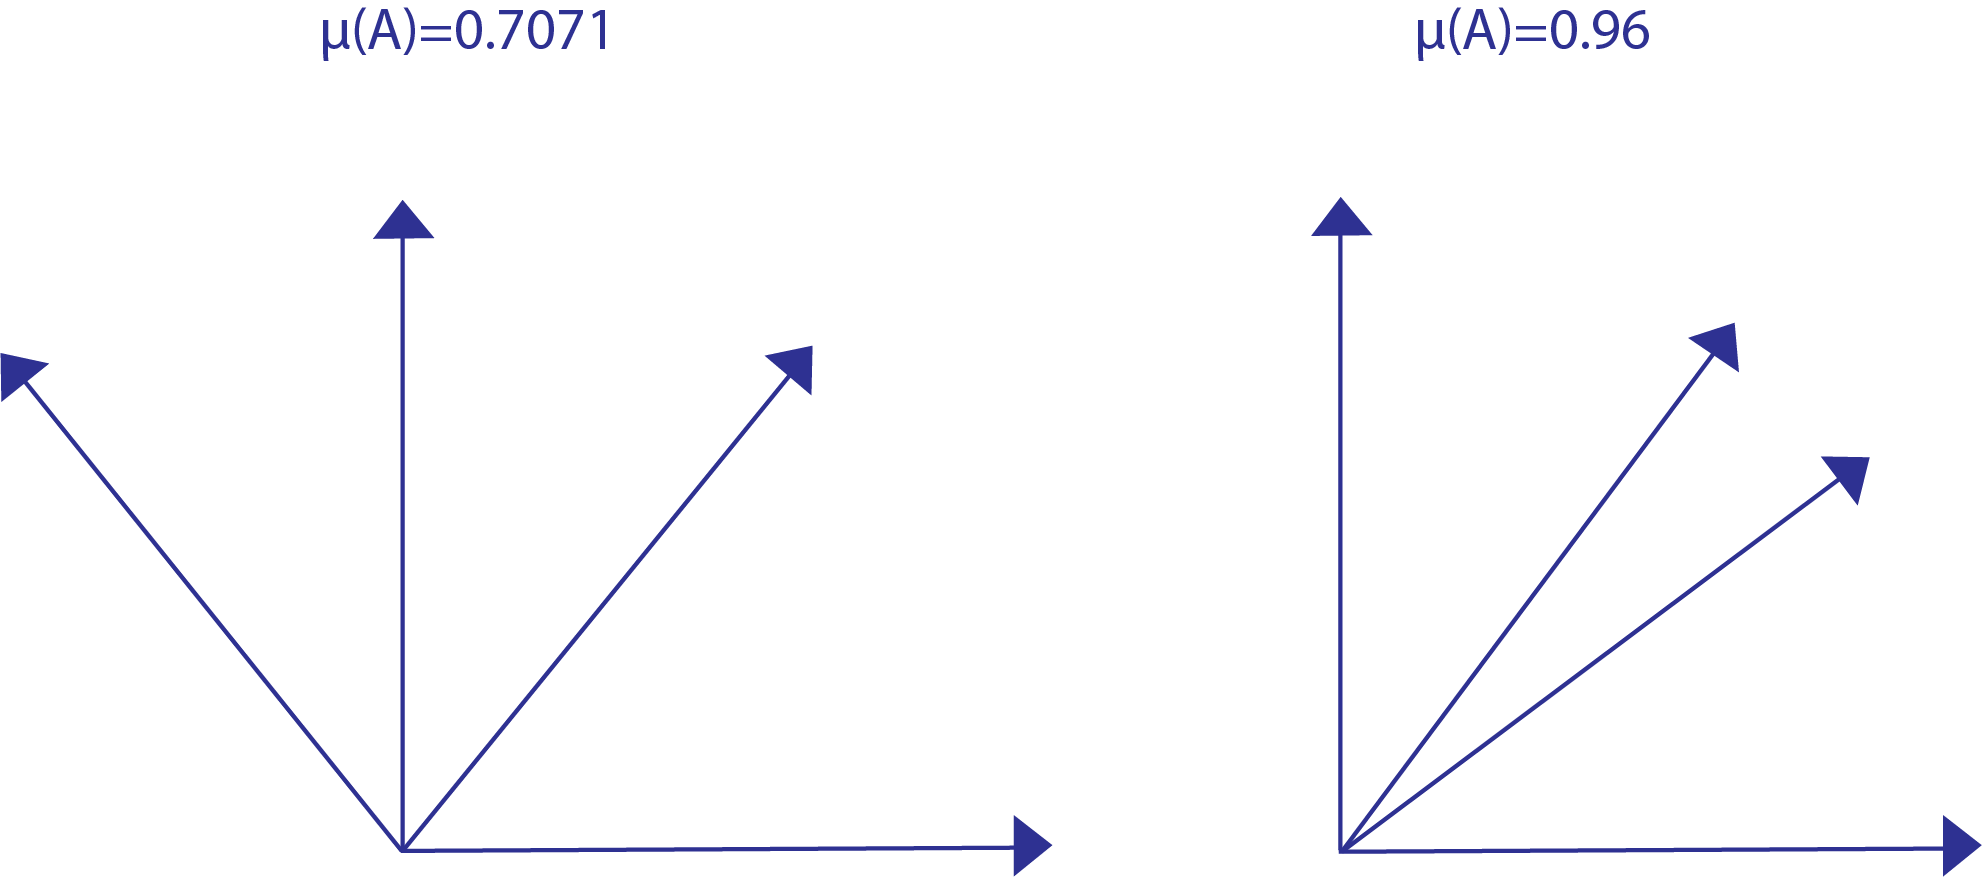
\includegraphics[scale = 0.7]{coherence_illustration_final.png}
    \caption{Visualization of a general coherence computation in $\BR^2$ for two sets of four unit vectors, based on a figure from Wright and Ma \cite{wm}. The left-hand set is spaced apart by $\frac{\pi}{4}$ radians each, and the right-hand set consists the two standard unit vectors and the vectors $(\frac{3}{5},\frac{4}{5})^\top$ and $(\frac{4}{5},\frac{3}{5})^\top$.}
    \label{coh-vis}
\end{figure}

The $\ell^1$-coherence function, which we more commonly use, and is more useful for recovery guarantees, is defined based on some sparsity $s$, and looks at a worst case cumulative dependence which is more important to consider.

\begin{Def}\label{cohthm} For a matrix $\bdA\in\BC^{m\times N}$ with $\ell^2$-normalized columns $\bda_1,...,\bda_N$ with $\|\bda_i\|=1,\forall i\in[N]$, the $\ell^1$ \textit{coherence} function, with argument $s\in[N-1]$, is

\begin{align}\label{cohsta}
    \mu_1(s):=\max_{i\in[N]}\left[\max_{S\subset[N]\backslash\{i\},\card(S)=s}\{\sum_{j\in S}|\langle \bda_i,\bda_j\rangle|\}\right].
\end{align}
\end{Def}

Note that we define coherence for matrices with $\ell^2$-normalized columns since we can always rescale the entries of the signal vector to obtain the appropriate response vector $\bdy$. This function measures the worst case scenario for the total dependence between one column of $\bdA$ and the columns of $\bdA$ from a disjoint index set of size $s$ \cite{fou-rau}. Initially this appears to be a complicated formula, but we can check that this function aligns with our intuitive understanding by seeing that for an orthogonal matrix, the coherence will be 0 for any sparsity $s$. Of course in our case for $m<N$, it is impossible to construct an orthogonal $m\times N$ matrix, so we have to rely on this concept of small worst case dependence between sparse sets and single other vectors.

Coherence ends up being a nice function to work with, and there are plenty of results for bounds on coherence, many of which are covered by Foucart and Rauhut \cite{fou-rau}. In particular, for any matrix $\bdA\in\BC^{m\times N}$ the coherence $\mu$ increases as $N$ increases and decreases as $m$ increases, but much faster in the latter case, given by the result that the coherence satisfies \cite{fou-rau}
\begin{align}\label{mu-lower}
    \mu\geq\sqrt{\frac{N-m}{m(N-1)}}.
\end{align}
In addition there is a relation between the general and $\ell^1$ coherence functions:
\begin{align}\label{mu-relation}
    \mu\leq\mu_1(s)\leq s\mu, \forall s\in[N-1].
\end{align}
See Appendix \ref{coh-ric} for a proofs of the results (\ref{mu-lower}) and (\ref{mu-relation}).

We care specifically about what the coherence of a matrix means for our ability to recover a sparse signal via $\ell^1$-minimization. In fact there is a relatively straightforward condition, which is given in the following theorem \cite{fou-rau}:

\begin{Th}\label{coh-thm} For $\bdA\in\BC^{m\times N}$ a matrix with $\ell^2$-normalized columns, if \begin{align}\mu_1(s)+\mu_1(s-1)<1\end{align} then every $s$-sparse $\bdx\in\BC^N$ is recovered exactly, both by basis pursuit (Section \ref{bp}), and orthogonal matching pursuit (Section \ref{omp}) after at most $s$ iterations.
\end{Th}

Basis pursuit and orthogonal matching pursuit are algorithms for compressed sensing, more detailed explanations for which are given in the associated sections, but for now note that basis pursuit is essentially shorthand for performing the $\ell^1$ minimization (\ref{l1}), and orthogonal matching pursuit is a greedy method that iteratively chooses an index set of size $s$, adding one new index to this set at each of its iterations. The following proof sketch is adapted from Foucart and Rauhut \cite{fou-rau}.

\begin{proof}
    First we sketch the proof for basis pursuit. This proof relies on Theorem \ref{bp-cond}, which says that to prove exact recovery via basis pursuit we need to prove the null space property of order $s$:
    \begin{align}\label{nsp-bp}
        \|\bdv_S\|_1<\|\bdv_{\bar S}\|_1,
    \end{align}
    where $S\subset[N]$ has $\card(S)=s$, $\bar S$ is the complement of $S$ in $[N]$, and $\bdv\in\ker(\bdA)$ is nonzero, which means $\bdv=\sum_{j\in[N]}v_j\bda_j$ for $\bda_j$ the $j$th column of $\bdA$. We want to bound $\|\bdv_S\|_1=\sum_{i\in S}|v_i|$, so let's look at $v_i$. Since $\bdv\in\ker(\bdA)$, we know
    \begin{align*}
        \left\langle\sum_{j=1}^Nv_j\bda_j,\bda_i\right\rangle=0\Rightarrow v_i=v_i\langle\bda_i,\bda_i\rangle=-\sum_{k\in\bar S}v_k\langle\bda_k,\bda_j\rangle-\sum_{j\in S,j\neq i}v_j\langle\bda_j,\bda_i\rangle.
    \end{align*}
    Thus using the triangle inequality we get that
    \begin{align*}
        |v_i|\leq\sum_{k\in\bar S}|v_k||\langle\bda_k,\bda_i\rangle|+\sum_{j\in S,j\neq i}|v_j||\langle\bda_j,\bda_i\rangle|,
    \end{align*}
    after which to get a bound on $\|\bdv_S\|_1$ we sum over all $i\in S$, getting
    \begin{align*}
        \|\bdv_S\|_1&\leq\sum_{k\in\bar S}|v_k|\sum_{i\in S}|\langle\bda_\ell,\bda_i\rangle|+\sum_{j\in S}|v_j|\sum_{i\in S,i\neq j}|\langle\bda_j,\bda_i\rangle|\\&\leq\sum_{k\in\bar S}|v_\ell|\mu_1(s)+\sum_{j\in S}|v_j|\mu_1(s-1)=\mu_1(s)\|\bdv_{\bar S}\|_1+\mu_1(s-1)\|\bdv_S\|_1.
    \end{align*}
    For this last inequality we used the fact that the coherence with argument $s$ is a maximum of $\sum_{i\in S}|\langle\bda_k,\bda_i\rangle|$ terms, over $\card(S)=s$ and $k\notin S$. We then re-arrange this inequality to obtain
    \begin{align*}
        \|\bdv_S\|_1(1-\mu_1(s-1))\leq\|\bdv_{\bar S}\|\mu_1(s),
    \end{align*}
    which becomes (\ref{nsp-bp}) when we apply the strict inequality $\mu_1(s)<1-\mu_1(s-1)$.\\
    
\end{proof}

\begin{proof}
    Second, we sketch the proof for orthogonal matching pursuit. For $(\bda_j)_{j\in[N]}$ the columns of $\bdA$, Proposition \ref{omp-cond} states that we need to prove that for any index set $S\subset[N]$ with $\card(S)=s$, that the matrix $\bdA_S$ of $\bdA$ on the support set $S$ is injective, and for all $\bdw=\bdA\bdx$ for $s$-sparse $\bdx$, 
    \begin{align*}
        \max_{j\in S}|\langle\bdw,\bda_j\rangle|>\max_{k\notin S}|\langle\bdw,\bda_k\rangle|.
    \end{align*}
    Denoting $\bdw=\sum_{i=S}w_i\bda_i$ for $w_i$ the nonzero coefficients of some $\bdx$, we see that for $k\notin S$,
    \begin{align*}
        |\langle\bdw,\bda_k\rangle|=\left|\sum_{i\in S}w_i\langle\bda_i,\bda_k\rangle\right|\leq\sum_{i\in S}|w_i||\langle\bda_i,\bda_k\rangle|\leq|w^*|\mu_1(s),
    \end{align*}
    using a simple triangle inequality, with $|w^*|=\max_{i\in S}|w_i|$ which exists since $S$ is a finite set, and since the computation for $\mu_1(s)$ is the max of $\sum_{i\in S}|\langle\bda_i,\bda_k\rangle|$ where $k\notin S$. Then for any $j\in S$, we have
    \begin{align*}
        |\langle\bdw,\bda_j\rangle|=\left|\sum_{i\in S}w_i\langle\bda_i,\bda_k\rangle\right|&\geq|w_j||\langle\bda_j,\bda_j\rangle|-\sum_{i\in S,i\neq j}|w_i||\langle\bda_i,\bda_j\rangle|\\&\geq|w_j|-|w^*|\mu_1(s-1),
    \end{align*}
    where the first inequality results from the triangle inequality applied to $w_j\langle\bda_j,\bda_j\rangle=\langle\bdw,\bda_j\rangle-\sum_{i\in S,i\neq j}w_i\langle\bda_i,\bda_j\rangle$, we use the fact that each $\bda_j$ is $\ell^2$ normalized to get that $\langle \bda_j,\bda_j\rangle=\|\bda_j\|_2^2=1$, and using the same bound on the coherence, this time for argument $s-1$. The maximum of these such values occurs when $w_j=w^*$, so 
    \begin{align*}
        |\langle\bdw,\bda_j\rangle|\geq|w^*|-|w^*|\mu_1(s-1)
    \end{align*}
    for all $j\in S$. Thus, by our assumption, $\mu_1(s)+\mu_1(s-1)<1$, so conclude that 
    \begin{align*}
        \max_{j\in S}|\langle\bdw,\bda_j\rangle|\geq|w^*|-|w^*|\mu_1(s-1)>|w^*|\mu_1(s)\geq\max_{k\notin S}|\langle\bdw,\bda_k\rangle|,
    \end{align*}
    which is what we wanted. The proof concludes with $\bdA_S$ being injective, which we won't include here but is a result of Corollary 5.4 in \cite{fou-rau}.
\end{proof}

Proofs of Theorem \ref{bp-cond} and Prop \ref{omp-cond} are given in Appendix \ref{bp-omp-conds} for the interested reader. This above proof is nice since it showcases why coherence is in many ways a natural metric and delineator between the support set $S$ and its complement $\bar S$.

We discuss exact formulations for orthogonal matching pursuit and basis pursuit later in Section \ref{algs}, but for now it suffices to note that simple conditions such as the above involving coherence allows for recovery for multiple different methods for performing $\ell^1$-minimization. Foucart and Rauhut additionally note that in order to obtain a matrix with low enough coherence to achieve recovery, the minimum number of measurements is on the order of $m\geq Cs^2$ \cite{fou-rau}.

We obtain this quadratic lower bound in $s$ for $m$ in particular using (\ref{mu-relation}). For a matrix with coherence bounded by $\mu\leq c/\sqrt{m}$ (which can be obtained reliably as shown in \cite{fou-rau}), we can get $\mu_1(s)+\mu_1(s-1)\leq(2s-1)\mu<1$ when $m>c^2(2s-1)^2$, which is on the order of $s^2$.

\subsection{Restricted Isometry Property}\label{rip-section}

While it may not be immediately obvious, this minimum number of measurements, while certainly a worst-case scenario, is suboptimal, as this worst case value for $m$ scales quadratically with the sparsity $s$, a bound known early in the field as the "quadratic bottleneck" \cite{fou-rau}. Overcoming this bottleneck was a major item of research at this time, and we are able to do so through introducing our next notion for the "niceness" of a matrix, called the \textit{restricted isometry property}. 

The restricted isometry property relies on the \textit{restricted isometry sonstant}, a measure similar in interpretation to coherence, as it concerns a worst case bound for the action of a matrix $\bdA$ restricted to an index set $S\subset[N]$. In this case the terminology is suitably descriptive, as the intuition is that matrices with small restricted isometry constant act like isometries (distance-preserving maps) on their restrictions to $s$-sparse vectors. In particular, we define the constant as a function of sparsity $s$ and implicitly of matrix $\bdA$.

\begin{Def}\label{ric} The \textit{restricted isometry constant} $\delta_s$ of a matrix $\bdA\in\BC^{m\times N}$ for sparsity $s$, is defined to be the smallest $\delta\geq0$ with, for all $s$-sparse $\bdx\in\BC^N$,
\begin{align}\label{ric-def}
    (1-\delta)\|\bdx\|_2^2\leq\|\bdA\bdx\|_2^2\leq(1+\delta)\|\bdx\|_2^2.
\end{align}
\end{Def}

Note that depending on the structure of the matrix $\bdA$, $\delta_s$ could take any value in the positive reals $[0,\infty)$, including $\delta_s>1$. The value $\delta_s$ has an equivalent formulation in terms of the matrix norm of $\bdA_S^*\bdA_S$ (where the $^*$ operator is the conjugate transpose and $\bdA_S$ is the restriction of $\bdA$ to index set $S$ with $\card(S)\leq s$) which measures its closeness to the identity and is given formally in Appendix \ref{ric-alt} \cite{fou-rau}. The measure's relationship to coherence is formalized in Appendix \ref{ric-coh}. 

We say that a matrix $\bdA$ satisfies the \textit{restricted isometry property} if, for large enough $s$, $\delta_s$ is small in some sense. This definition is rather informal, as there is no neat statement of the restricted isometry property, but our takeaway is rather the general idea that we will be able to prove guarantees that rely on a bound on $\delta_s$ based on the size of $s$.

The notion of smallness for $\delta_s$ gives way, as we might hope, to reconstruction guarantees for our algorithms. The following result, which is the main result on which we focus, is very simple and quite beautiful. For basis pursuit (\ref{bp}) we have the following theorem, involving the $2s$th restricted isometry constant $\delta_{2s}$.

\begin{Th}\label{ric-bp} If the $2s$th restricted isometry constant of the matrix $\bdA\in\BC^{m\times N}$ satisfies
\begin{align}
    \delta_{2s}<\frac{1}{3},
\end{align}
then every $s$-sparse $\bdx\in\BC^N$ is the unique solution to the $\ell^1$-minimization (\ref{l1}), in that it is recovered exactly from the minimization problem
\begin{align*}
    \textnormal{minimize }\|\bdz\|_1 \ \ \textnormal{subject to }\bdA\bdz=\bdA\bdx.
\end{align*}
\end{Th}

We will give a sketch of the proof of this important theorem, which will draw on results from \cite{fou-rau}, and will hopefully give a bit of intuition for why the very nice bound of $\delta_{2s}<\frac{1}{3}$ comes up.

\begin{proof} 
    As with the proof of Theorem \ref{coh-thm} in the basis pursuit case, we make use of Prop \ref{bp-cond} and specifically the reformulation of the null space property (\ref{nsp-ref}) that says we must prove that $\|\bdv_S\|_1\leq\frac{1}{2}\|\bdv\|_1$ for any nonzero $\bdv\in\ker(\bdA)$ and $S\subset[N]$ with $\card(S)=s$. This proof relies on showing this version of the null space property through a stronger condition,
    \begin{align}\label{stronger}
        \|\bdv_S\|_2\leq\frac{\rho}{2\sqrt{s}}\|\bdv\|_1,
    \end{align}
    on the same inputs as for (\ref{nsp-ref}), and defining
    \begin{align*}
        \rho:=\frac{2\delta_{2s}}{1-\delta_{2s}}.
    \end{align*}
    We see that (\ref{stronger}) implies (\ref{nsp-ref}) since $\|\bdv_S\|_1\leq\sqrt{s}\|\bdv_S\|_2$ from the properties of the $\ell^1$ and $\ell^2$ balls and norms, and $\rho<1$ as long as $\delta_{2s}<\frac{1}{2}$, which is one of our hypotheses. It is because of this formulation that the upper bound of $\frac{1}{3}$ for $\delta_{2s}$ is given.
    
    The key to this proof, which will not give fully, is to partition the index set $[N]$ into a sequence of sets $S=:S_0,S_1,S_2,...$ with $S_k$ being the $s$ indices in $\overline{S_0\cup\cdots\cup S_{k-1}}$ with the largest absolute entries of $\bdv$. Then our goal is to bound $\|\bdv_S\|_1=\|\bdv_{S_0}\|_1$, which we do first through the definition of $\delta_s$ (\ref{ric-def}), and the fact that $\delta_{2s}\leq\delta_s$:
    \begin{align*}
        \|\bdv_{S_0}\|^2_2\leq\frac{1}{1-\delta_{2s}}\|\bdA\bdv_{S_0}\|^2_2&=\frac{1}{1-\delta_{2s}}\langle\bdA\bdv_{S_0},-\bdA\bdv_{S_1}-\bdA\bdv_{S_2}-\cdots\rangle\\&=\frac{1}{1-\delta_{2s}}\sum_{k\geq1}\langle\bdA\bdv_{S_0},\bdA(-\bdv_{S_k})\rangle.
    \end{align*}
    Combined with the fact (from Corollary 6.3 in \cite{fou-rau} which we give without proof) that $\langle\bdA(\bdv_{S_0}),\bdA(-\bdv_{S_k})\rangle\leq\delta_{2s}\|\bdv_{S_0}\|_2\|\bdv_{S_k}\|_2,$ and after dividing by $\|\bdv_{S_0}\|_2$, we get:
    \begin{align*}
        \|\bdv_{S_0}\|_2\leq\frac{\rho}{2}\sum_{k\geq1}\|\bdv_{S_k}\|_2\leq\frac{\rho}{2\sqrt{s}}\sum_{k\geq1}\|\bdv_{S_{k-1}}\|_1\leq\frac{\rho}{2\sqrt{s}}\|\bdv_{S_0}\|_1,
    \end{align*}
    where we used without proof Lemma 6.10 from \cite{fou-rau}, which says that 
    \begin{align*}\|\bdv_{S_k}\|_2\leq\frac{1}{\sqrt{s}}\|\bdv_{S_{k-1}}\|_1.
    \end{align*}
    At this point we are done.
    
\end{proof}

For more complete proofs of Corollary 6.3 and Lemma 6.10 from \cite{fou-rau} we refer the reader to Foucart and Rauhut, but to give a bit of intuition, Corollary 6.3 follows from the properties of the restricted isometry constant on the set $S_0\cup S_k$ of size $2s$ (hence why the restricted isometry constant $\delta_{2s}$ shows up). Lemma 6.10 has a geometric proof based on the fact that each absolute entry of $\bdv_{S_{k-1}}$ is greater than each absolute entry of $\bdv_{S_k}$.

This condition sounds almost too good to be true, but it is more so just a clean result which is easy to remember; it is in fact possible to make the upper bound larger and thus more optimal \cite{fou-rau}. Nevertheless, it remains that using the restricted isometry property in basis pursuit has its limitations, among which is the fact that adding or otherwise shuffling and scaling the measurements can interfere with the restricted isometry constant. In particular, adding a measurement can increase the constant, though we might intuitively guess that adding a measurement would increase the chance of recovery \cite{fou-rau}.

\subsection{Recovery with Random Matrices}\label{random-matrix}

As mentioned, the quadratic bottleneck unfortunately comes up when framing a matrix in terms of coherence, but it turns out that we can beat this limitation through the restricted isometry constant with the following minimum number of measurements \begin{align*} m\geq C_\delta s\ln(eN/s),\end{align*} which will guarantee a restricted isometry constant $\delta_s\leq\delta$ in a random setting which we will define. Here $C_\delta$ is a constant depending on a chosen constant $\delta$, our intended upper bound on the restricted isometry constant, and $e$ is the standard notation for Euler's constant $e\approx2.718$, and is present as a shorthand for saying $m$ is bounded from below by an $s+s\ln(N/s)$ term. As it turns out, proving that certain deterministic matrices meet the requirements to have this optimal lower bound for the number of measurements is a difficult task, with research into this task currently ongoing \cite{fou-rau}. As such, the breakthrough in compressed sensing came with the advent of using random measurement matrices. 

Specifically, the most common random matrices used are Gaussian random matrices. Gaussian random matrices are defined as matrices $\bdA\in\BR^{m\times N}$ with each entry an independent standard Gaussian $\mathcal{N}(0,1)$, which is a random variable with mean 0 and variance 1. The Gaussian distribution is also known as the normal distribution. The probability density function (PDF) of the Gaussian distribution is 
\begin{align*}
    f(x)=\frac{1}{\sqrt{2\pi}}\exp(-\frac{x^2}{2}),
\end{align*}
and the cumulative distribution function (CDF) for $X\sim\mathcal{N}(0,1)$ is $F(x)=\BP(X\leq x)=\int_{-\infty}^xf(x)dx$ which is usually notated as $\Phi(x)$ since the partial integral does not have a closed form. The PDF is symmetric about the origin, with heavy tails, and as such the Gaussian PDF is often referenced as a "bell curve". See Figure \ref{density-plot} in Section \ref{sim-matrix} for a plot of this PDF.

Commonly, the $\ell^2$-normalized version of such a matrix $\frac{1}{\sqrt{m}}\bdA$ is taken, so for any column $\bda_i$ of $\bdA$, $$\BE(\|\frac{1}{\sqrt{m}}\bda_i\|^2_2)=\frac{1}{m}\sum_{j=1}^m\BE(\bda_{ij}^2)=1,$$ since each $\bda_{ij}\sim\mathcal{N}(0,1)$ independently so $\BE(\bda_{ij}^2)=\var(\bda_{ij})+\BE(\bda_{ij})^2=1+0=1$. Note that we have that $\frac{1}{\sqrt{m}}\bdA$ is $\ell^2$-normalized in the sense that the \textit{square} of the $\ell^2$ norm of each column is 1 in expectation. From Jensen's inequality, which says that for convex $g:\BR\rightarrow\BR$, $g(E(X))\leq E(g(X))$, we know that $\BE(\|\frac{1}{\sqrt{m}}\bda_i\|_2)^2\leq\BE(\|\frac{1}{\sqrt{m}}\bda_i\|^2_2)$, but scaling by $\frac{1}{\sqrt{m}}$ is easy and turns out to be good enough, as we will see in Section \ref{gaussian-pf}.

Another distribution over which measurement matrices are taken is often called the Bernoulli random matrix, which counter-intuitively does not have Bernoulli entries but rather independent Rademacher entries. Thus the entries take $1$ or $-1$ with equal probability $\frac{1}{2}$ (the confusion is since Bernoulli random \textit{variables} are usually given as taking the values of 1 or 0 with equal probability $\frac{1}{2}$). To minimize confusion we will simply call such matrices Rademacher random matrices, to emphasize that their entries are independent Rademacher random variables, which have PMF
\begin{align*}
    f(x)=\begin{cases}
        \frac{1}{2} & x = 1 \\
        \frac{1}{2} & x = -1 \\
        0 & \text{otherwise}.
    \end{cases}
\end{align*}
More generally, compressed sensing works with a class of random matrices defined as subgaussian, a class in which both Gaussian and Rademacher random matrices fall \cite{fou-rau}. This terminology is based on the class of subgaussian random variables, which include Gaussian and Rademacher random variables.

\begin{Def} A random variable $X$ is \textit{subgaussian} if there are constants $\beta,\kappa>0$ with
\begin{align}
    \BP(|X|\geq t)\leq\beta e^{-\kappa t^2} \ \ \forall t>0.
\end{align}
\end{Def}

The left hand side quantity we are bounding is the often called the reverse-CDF of $X$ (with reference to the CDF $F(t)=\BP(X\leq t)$), and we can think of subgaussian random variables as those for which the log of their reverse CDF is quadratic in $t$ in the sense that it is bounded above by $-t^2$ up to a constant factor. Examples of subgaussian random variables include the Gaussian, which is subgaussian with parameters $\beta=1,\kappa=1/2$, as well as Rademacher random variables and all almost surely bounded random variables. These variables are classified together in this way due to the behavior of their tails, which allow them to satisfy many nice properties. They contrast with subexponential random variables, which have fatter tails, a la the exponential distribution. Note that while subexponentials have heavier tails, both subgaussians and subexpontentials broadly speaking have light tails since their reverse CDFs approach zero exponentially in the positive direction. See Section \ref{sim-matrix} for a comparison of compressed sensing using subgaussian versus subexponential matrices. The definition of subgaussian random variables is naturally extended to random matrices in the same way as we defined for Gaussian and Rademacher matrices.

\begin{Def}\label{subgaussian} A matrix $\bdA\in\BR^{m\times N}$ is a \textit{subgaussian} random matrix if it has independent subgaussian entries with mean 0 and the same subgaussian parameters $\beta,\kappa$.
\end{Def}

Important to note is that the entries of such a subgaussian $\bdA$ are all independent and identically distributed, with the same parameters. Specifying the subgaussian parameters $\beta,\kappa$ is the most common way to define a general subgaussian distribution \cite{fou-rau}.

With this set of random matrices in mind, we see a path to the achievement of the optimal restricted isometry property through the following theorem.

\begin{Th}\label{rip-subg} For $\bdA\in\BR^{m\times N}$ a subgaussian matrix, there exists a constant $C$ depending only on the parameters of the subgaussian distribution ($\beta,\kappa$) where the restricted isometry constant of $\frac{1}{\sqrt{m}}\bdA$ satisfies $\delta_s\leq\delta$ with probability at least $1-\varepsilon$, as long as
\begin{align}
    m\geq C\delta^{-2}(s\ln(eN/s)+\ln(2\varepsilon^{-1})).
\end{align}
\end{Th}

Theorem \ref{rip-subg} provides a criterion for ensuring that the $s$th restricted isometry constant $\delta_s$ of the matrix $\frac{1}{\sqrt{m}}\bdA$ is below a certain desired threshold $\delta$ with high probability. Theorem \ref{ric-bp} tells us that bounding the restricted isometry constant provides for sparse recovery, so finding this criterion is an essential step toward recovery with random matrices that we will complete in the following theorem, which corresponds to a recovery condition in the $\ell^1$-minimization problem (\ref{l1}).

\begin{Th}\label{rip-l1} For $\bdA\in\BR^{m\times N}$ a subgaussian matrix, and $\varepsilon\in(0,1)$, there exist parameters $C_1,C_2>0$ depending on the subgaussian parameters ($\beta,\kappa$) such that if
\begin{align}\label{rip-l1-ineq}
    m\geq C_1s\ln(eN/s)+C_2\ln(2\varepsilon^{-1}),
\end{align}
then with probability at least $1-\varepsilon$, any $s$-sparse $\bdx\in\BR^N$ is the unique solution to the $\ell^1$-minimization (\ref{l1}).
\end{Th}

The proof of Theorem \ref{rip-l1} follows from applying Theorem \ref{rip-subg} and Theorem \ref{ric-bp}, which combine to remove the $\delta$ parameter in (\ref{rip-l1-ineq}). The proof of Theorem \ref{rip-subg} is more engaged, involving numerous intermediate lemmas and theorems in \cite{fou-rau}, which the reader can consult for the complete picture. We will prove a simpler version of these results in Section \ref{gaussian-pf} for Gaussian matrices, which will more clearly show why each term of the lower bound for $m$ is required.

Note that this recovery is first and foremost probabilistic, and the higher we want the probability of recovery the larger we must make $m$ (via decreasing $\varepsilon$). In addition, note that the use of two constants $C_1,C_2$ as opposed to just $C$ in Theorem \ref{rip-subg} conveys fundamentally the same condition, but we can make the minimum number of measurements smaller with the two constants, which is more helpful in practice.

These recovery conditions take the form of \textit{uniform} recovery, which is when all $s$-sparse vectors $\bdx$ are recoverable from $\bdA$ with high probability, whereas \textit{non-uniform} recovery concerns the probability that any given $s$-sparse vector can be recovered. This weaker condition is often easier to achieve, so it has its place in the literature, though we will not cover it any further \cite{fou-rau}.

\subsection{Proof of the Restricted Isometry Property for Gaussian Matrices}\label{gaussian-pf} Concluding the satisfaction of the restricted isometry property for random matrices as a black box is somewhat unsatisfying, especially since the development is such an important part of the start of compressed sensing as a field. The proof relies on various concentration inequalities for subgaussian distributions, which are somewhat advanced probabilistic tools, and the proof is additionally involved as the subgaussian is general, with two constants $\beta$ and $\kappa$ \cite{fou-rau}. The reader may refer to Foucart and Rauhut's textbook \textit{A Mathematical Introduction to Compressed Sensing} \cite{fou-rau} for a more complete proof of Theorems \ref{rip-subg} and \ref{rip-l1}, which as mentioned primarily makes use of concentration inequalities on the tails of subgaussian distributions.

However, the standard Gaussian distribution is very well-known and understood, and a proof of the restricted isometry property for a Gaussian matrix requires only basic facts about the Gaussian distribution and the Chernoff bound, whic hare standard results in introductory probability. Thus we will include a proof of Theorem \ref{rip-subg} specifically for Gaussian random matrices that will paint an illuminating picture of the nature of the restricted isometry property.

\begin{Th}\label{rip-gaussian} The matrix $\bdA\in\BR^{m\times N}$, a normalized Gaussian matrix, with i.i.d. $\bdA_{ij}\sim\mathcal{N}(0,\frac{1}{m})$ entries, satisfies the restricted isometry property with restricted isometry constant $\delta_s\leq\delta$ with probability $1-\varepsilon$ if
\begin{align}\label{rip-gaussian-m}
    m\geq\frac{2s\log(eN/s)+2\log(2\varepsilon^{-1})}{\delta-\log(\delta+1)}.
\end{align}

\end{Th}

For this proof we draw on \cite{fou-rau, park-lee}, as well as basic results from introductory probability theory.

\begin{proof}
    In order to first compute the restricted isometry constant $\delta_s(\bdA)$, we need to find the smallest $\delta'$ such that for all $s$-sparse $\bdx$, 
    
    \begin{align}\label{rip-delta'}
        (1-\delta')\|\bdx\|_2^2\leq\|\bdA\bdx\|_2^2\leq(1+\delta')\|\bdx\|_2^2.
    \end{align}
    
    Here everything is held constant except for $\bdA$, which is random in the way given, meaning $\|\bdA\bdx\|_2^2$ is a random variable taking values $\BR$. In particular, 
    \begin{align*}
        \|\bdA\bdx\|_2^2=\sum_{i=1}^m|\langle\bda_i,\bdx\rangle|^2,
    \end{align*}
    where for $\bda_i$ the $i$th row of $\bdA$, the inner product (which is just the dot product in this real setting) is $\langle\bda_i,\bdx\rangle=\sum_{j=1}^N\bda_{ij}\bdx_j\sim\mathcal{N}(0,\frac{\|\bdx\|_2^2}{m})$ using the standard properties of a linear combination of Gaussian variables, where $\|\bdx\|_2^2=\sum_{j=1}^N\bdx_j^2$. Then $\|\bdA\bdx\|_2^2$ is a sum of $m$ squared Gaussians, meaning $\|\bdA\bdx\|_2^2\sim\frac{\|\bdx\|_2^2}{m}\cdot\chi_m^2$ for $\chi_m^2$ a standard $\chi^2$ (Chi-squared) random variable with $m$ degrees of freedom. Then if we want to bound the probability that (\ref{rip-delta'}) holds for $\delta$, we want to bound $\BP(|\|\bdA\bdx\|_2^2-\|\bdx\|_2^2|\leq\delta\|\bdx\|_2^2)$ from below. From the distribution we derived for $\|\bdA\bdx\|_2^2$ we know that
    \begin{align*}
        \BE\left[\|\bdA\bdx\|_2^2\right]=\frac{\|\bdx\|_2^2}{m}\cdot m=\|\bdx\|_2^2,
    \end{align*}
    since the $\chi_m^2$ expectation is $m$ \cite{park-lee}, so bounding the complement of this probability from above is a natural strategy using basic concentration bounds from probability theory. Using the Chernoff bound (which is a standard probabilistic tool \cite{park-lee}) with a generic $t>0$ on random variable $\|\bdA\bdx\|_2^2$ and constant $\|\bdx\|_2^2(1+\delta)$, we obtain an upper bound of 
    \begin{align*}
        \BP(\|\bdA\bdx\|_2^2\geq\|\bdx\|_2^2(1+\delta))\leq\frac{\BE\left[\exp(t\|\bdA\bdx\|_2^2)\right]}{\exp(t\|\bdx\|_2^2(1+\delta))}=\frac{\left(1-\frac{2t\|\bdx\|_2^2}{m}\right)^{-m/2}}{\exp(t\|\bdx\|_2^2(1+\delta))},
    \end{align*}
    which is a result of the moment generating function (defined as $M(t)=\BE\left[\exp(tX)\right]$ for random variable $\bdX$) of the $\chi_m^2$ distribution \cite{park-lee}. In the same vein as the standard probability trick, we can minimize this upper bound as a function of $t$, since this is true for all $t>0$. We omit the computation, which is a matter of simple calculus, and yields 
    \begin{align*}
        t=\frac{m}{2\|\bdx\|_2^2}\left(\frac{\delta}{1+\delta}\right).
    \end{align*}
    Upon substituting this value of $t$, we retrieve the bound
    \begin{align}\label{bound-upper}
        \BP(\|\bdA\bdx\|_2^2\geq\|\bdx\|_2^2(1+\delta))\leq\frac{\left(1-\frac{\delta}{1+\delta}\right)^{-m/2}}{\exp(-m\delta/2)}=\exp\left(-m\delta/2\right)(1+\delta)^{m/2},
    \end{align}
    which is the upper part of our bound and the first half of $\BP(|\|\bdA\bdx\|_2^2-\|\bdx\|_2^2\geq\delta\|\bdx\|_2^2)$. Now we want to upper bound the lower probability $\BP(\|\bdA\|_2^2\leq\|\bdx\|_2^2(1-\delta))$. This formulation is not equipped for the same form of the Chernoff bound used earlier, but taking the negation before exponentiation gives an alternative formulation of the Chernoff bound for a random variable $X$:
    \begin{align*}
        \BP(|\bdX|\leq a)\leq\frac{\BE\left[\exp(-t|\bdx|)\right]}{\exp(-ta)}.
    \end{align*}
    Using this formulation, we obtain the bound
    \begin{align*}
        \BP(\|\bdA\bdx\|_2^2\leq\|\bdx\|_2^2(1-\delta))\leq\frac{\left(1+\frac{2t\|\bdx\|_2^2}{m}\right)^{-m/2}}{\exp(-ts(1-\delta))},
    \end{align*}
    since we are essentially just substituting $-t$ for $t$ and $(1-\delta)$ for $(1+\delta)$, meaning the moment generating function computation still works, and furthermore the minimizing value of $t$ is
    \begin{align*}
        t=-\frac{m}{2\|\bdx\|_2^2}\left(\frac{\delta}{1-\delta}\right),
    \end{align*}
    meaning we have after substitution:
    \begin{align}\label{bound-lower}
        \BP(\|\bdA\bdx\|_2^2\leq\|\bdx\|_2^2(1-\delta))\leq\exp(m\delta/2)(1-\delta)^{m/2}.
    \end{align}
    Combining (\ref{bound-upper}) and (\ref{bound-lower}) we obtain
    \begin{align*}
        \BP(|\|\bdA\bdx\|_2^2-\|\bdx\|_2^2\geq\delta\|\bdx\|_2^2)&\leq\exp\left(-m\delta/2\right)(1+\delta)^{m/2}+\exp(m\delta/2)(1-\delta)^{m/2}\\&\leq2\left(-m\delta/2\right)(1+\delta)^{m/2},
    \end{align*}
    since the numerical value of the former upper bound is the higher value \cite{park-lee}.
    
    This is the probability bound for a single $\bdx$, but in order to satisfy the restricted isometry property with $\delta_s\leq\delta$, we need this bound to be true for all $s$-sparse $\bdx$, of which there are $\binom{N}{s}$, so by a union bound, we obtain
    \begin{align*}
        \BP(|\|\bdA\bdx\|_2^2-\|\bdx\|_2^2\geq\delta\|\bdx\|_2^2,\forall\bdx\in V_s)&\leq2\binom{N}{s}\left(-m\delta/2\right)(1+\delta)^{m/2}\\&\leq2\left(\frac{eN}{s}\right)^s\left(-m\delta/2\right)(1+\delta)^{m/2},
    \end{align*}
    using the classic bound for a binomial coefficient $\binom{n}{k}\leq\left(\frac{en}{k}\right)^k$ \cite{park-lee}.
    
    We want this upper bound to be $\leq\varepsilon$ in order to conclude that $\bdA$ satisfies $\delta_s\leq\delta$ with probability at least $1-\varepsilon$, so we solve the following inequality for $m$:
    \begin{align*}
        2\exp(-\frac{m}{2}(\delta-\log(\delta+1))+s\log(eN/s))\leq\varepsilon.
    \end{align*}
    After taking the log of each side, it becomes a linear inequality in $m$ which is simple to solve, and gives us exactly the inequality (\ref{rip-gaussian-m}) which was assumed so we indeed conclude that $\delta_s\leq\delta$ with probability $\geq1-\varepsilon$.
    
\end{proof}

Hopefully this proof gives a good intuition for why Gaussian variables in particular are good candidates for satisfying the restricted isometry property, specifically as a result of their short tails. However, note that other short-tailed distributions (i.e. those whose reverse CDFs decay exponentially) do not produce the same results as Gaussians or subgaussians, notably the Exponential and corresponding subexponential family \cite{fou-rau}. To visualize the difference in sparse recovery performance between random matrices of each type, see Section \ref{sim-matrix} for a brief simulated comparison.

\section{Algorithms for Sparse Recovery}\label{algs}

With a field such as compressed sensing, where much of its value lies in performing a recovery with as few measurements as possible, we naturally care about the ease of implementation in practice with real data, and thus the field is entwined with algorithmic design. We've already seen in Section \ref{theory} that recovery guarantees are usually framed in terms of their corresponding algorithms, including basis pursuit and orthogonal matching pursuit. 

In this section we detail the various types of algorithms which have been used in the field, which fall into three major categories: convex optimization (Section \ref{bp}), greedy algorithms (Section \ref{omp}), and thresholding algorithms (Section \ref{thresh}). We will also compare via simulation the performance of these algorithms based on the number of measurements and sparsity of the problem in Section \ref{omp-bp-comparison} and compare how the choice of measurement matrix impacts recovery rate in Section \ref{sim-matrix}.

\subsection{Convex Optimization via Basis Pursuit}\label{bp}

The first and most intuitive algorithm we give is basis pursuit. Below is the pseudocode for basis pursuit (BP), which is actually somewhat useless because it is actually just saying to perform the $\ell^1$-minimization problem (\ref{l1}).

\begin{algorithm}
 \textit{Input:} measurement matrix $\bdA$, response vector $\bdy$\;
 \textit{Do:} $\bdx^*=\argmin||\bdz||_1 \text{ with }\bdy=\bdA\bdz$\;
 \textit{Output:} The vector $\bdx^*$.
 \caption{Basis Pursuit}
\end{algorithm}

Here $\argmin$ entails choosing the vector $\bdz\in\BC^N$ with $\bdy=\bdA\bdz$ that has a minimal $\ell^1$ norm. Basis pursuit is no more than the $\ell^1$-minimization problem (\ref{l1}), but its implementation is the more interesting question, which involves algorithms like linear programming, which constitute, for a set of problems with linear constraints, many well-documented ways of computing a solution. In Appendix \ref{lin-prog} we describe how to formulate basis pursuit via linear programming and a general intuition for how the computation method works.

\subsection{Greedy Solutions via Orthogonal Matching Pursuit}\label{omp}

The following is the pseudocode for orthogonal matching pursuit (OMP), which iteratively updates running counters for the candidate signal $\bdx^n$ and support set for $\bdx^n$, $S^n$. Note that $\bdA^*$ is notation for the adjoint matrix, or conjugate transpose, of $\bdA$.

\begin{algorithm}
 \textit{Input:} measurement matrix $\bdA$, response vector $\bdy$, max sparsity $\bar n$\;
 \textit{Initialize:} $\bdx^0=\mathbf{0},S^0=\varnothing$\;
 \textit{Iterate:} until $n=\bar n$;
 \begin{align*}
     S^{n+1}:=S^n\cup\{j_{n+1}\}, j_{n+1}:=\argmax_{j\in[N]}\{|\bdA^*(\bdy-\bdA\bdx^n)_j|\}\\
     \bdx^{n+1}:=\argmin_{\supp(\bdz)\subset S^{n+1}}\{||\bdy-\bdA\bdz||_2\};
 \end{align*}
\textit{Output:} $\bdx^*=\bdx^{\bar n}$.
 \caption{Orthogonal Matching Pursuit}
\end{algorithm}

The input $\bar n$ is the maximum number of iterations we will allow the algorithm to run, and is usually set to our target sparsity $s$ if it is known.

Parallel to the function of $\argmin$ for basis pursuit, here $\argmax$ entails choosing the index $j\in[N]$ with the maximal value of $|\bdA^*(\bdy-\bdA\bdx^n)_j|$, where $\bdA^*(y-\bdA-\bdA\bdx^n)_j$ is the $j$th element of the matrix $\bdA^*(y-\bdA-\bdA\bdx^n)$. Unlike basis pursuit, which is a simple restatement of $\ell^1$-minimization, there is more explanation required to reason why orthogonal matching pursuit should at least be a suitable proxy for $\ell^1$-minimization. The following lemma and associated proof help to explain why the index added at each step is optimal.

\begin{Lemma}\label{omp-lem} For $\bdA\in\BC^{m\times N}$ a matrix with $\ell^2$-normalized columns, and given $S\subset[N]$, $\bdv$ with $\supp(\bdv)=S$, and $j\in [N]$, if
\begin{align}\label{omp-min}
    \bdw := \argmin_{\supp(\bdz)\subset S\cup\{j\}}\{||\bdA\bdz-\bdy||_2\}
\end{align}
then
\begin{align}
    ||\bdA\bdw-\bdy||^2_2\leq||\bdA\bdv-\bdy||^2_2-|(\bdA^*(\bdy-\bdA\bdv))_j|^2.
\end{align}
\end{Lemma}

Treating $\bdx^n$ as $\bdv$, and $\bdx^{n+1}$ as $\bdw$, we see that Lemma \ref{omp-lem} tells us that choosing $j_{n+1}$ to maximize $|(\bdA^*(\bdy-\bdA\bdv))_j|^2$ will be optimal in minimizing the upper bound on $||\bdA\bdw-\bdy||_2$. At each iteration, the algorithm for orthogonal matching pursuit chooses a new index $j_{n+1}$ to add to the index set $S^n$ to decrease $||\bdA\bdx^n-\bdy||_2$ by as much as possible.

\begin{proof}
    In computing (\ref{omp-min}), we see that any $\bdz=\bdv+t\bde_j$ is supported on $S\cup\{j\}$, so $||\bdA\bdw-\bdy||_2\leq\min_{t\in\BC}||\bdA(\bdv+t\bde_j)-\bdy||_2$, at which point we can further bound the left side by taking $t=\rho e^{i\theta}$ as a generic complex number:
    \begin{align*}
    \begin{split}
        ||\bdA\bdv+t\bdA\bde_j-\bdy||^2_2&=||\bdA\bdv-\bdy||^2_2+||t\bdA\bde_j||^2_2-\Rea(\bar t\langle\bdA\bde_j,\bdA\bdv-\bdy\rangle)\\&=||\bdA\bdv-\bdy||_2^2+\rho^2-2\Rea(\rho e^{-i\theta}(\bdA^*(\bdy-\bdA\bdv))_j)\\&\geq||\bdA\bdv-\bdy||_2^2+\rho^2-2\rho|(\bdA^*(\bdy-\bdA\bdv))_j|,
    \end{split}
    \end{align*}
    from the fact that $||\bdA\bde_j||_2=1$ since the columns of $\bdA$ are $\ell^2$-normalized, and where the closing inequality comes from the fact that the real part of a complex vector is no greater than its magnitude. The optimal bound then results from choosing $t$ to minimize this expression, which is a quadratic polynomial in $\rho$, and completing the square gives the minimizing value of $\rho$ as $|(\bdA^*(\bdy-\bdA\bdv))_j|$, producing our final, intended inequality
    \begin{align*}
        ||\bdA\bdw-\bdy||^2_2\leq\min_{t\in\BC}||\bdA(\bdv+t\bde_j)-\bdy||^2_2=||\bdA\bdv-\bdy||_2-|(\bdA^*(\bdy-\bdA\bdv))_j|^2.
    \end{align*}
\end{proof}

In summary, orthogonal matching pursuit at each step chooses a new index $j_{n+1}$ which will decrease the $\ell^2$ norm distance between the response measurement $\bdy$ and the image under $\bdA$ of the candidate signal $\bdx^n$, and then the new candidate signal $\bdx^{n+1}$ is chosen on the new support set by minimizing this $\ell^2$ norm difference. It is in this sense that orthogonal matching pursuit is "greedy", since at each iteration in the algorithm it chooses a new index that maximizes its utility at the present step, without regard to any long term behavior, though we will see that orthogonal matching pursuit does turn out to perform rather well in general.

The benefits and downsides of orthogonal matching pursuit in comparison to basis pursuit are somewhat intuitive: because of its greedy nature and use of the $\ell^2$ norm orthogonal matching pursuit is faster and easier to implement than basis pursuit, but it is able to correctly recover a given signal less often than basis pursuit, that is to say in fewer situations. Nevertheless, orthogonal matching turns out to be a suitable replacement for basis pursuit, with similar enough recovery that its improvements in run time outpace its negatives. Kunis and Rauhut obtained this result for sparse recovery specifically for the data structure of trigonometric polynomials in 2008 \cite{kunis-rauhut}, and Tropp and Gilbert in 2007 similarly obtained a performance for orthogonal matching pursuit which was close to basis pursuit for the general experimental setting \cite{tropp-gilbert}. As perhaps the two most common approaches for compressed sensing, we will give a comparison of their performances on a generated dataset in section \ref{omp-bp-comparison}, in a fashion similar to Tropp and Gilbert's simulations.

While orthogonal matching pursuit is the most common greedy algorithm, others exist, such as compressive sampling matching pursuit (CoSaMP) \cite{fou-rau}, as well as hybrid methods combining greedy methods with convex optimization \cite{narayanan}. Next we will briefly overview a final major category of compressed sensing algorithms.

\subsection{Thresholding Methods for Sparse Recovery}\label{thresh}

Basis pursuit involves literally performing the $\ell^1$-minimization problem (\ref{l1}) and orthogonal matching pursuit is an intuitive greedy solution for recovering sparse signals, but there is a third major category of algorithms used in compressed sensing, known as thresholding algorithms. The method broadly speaking seeks to achieve the task of sparse recovery, which is essentially an inverse operation, by using the adjoint matrix $\bdA^*$ \cite{fou-rau}.

We will not delve too far into thresholding algorithms, but we will give some pseudocode for the most basic form of thresholding to provide some intuition for how they operate. First we define the function $L_s(\bdz)$ being the set of $s$ indices $i$ with the largest values of $|\bdz_i|$ for $\bdz\in\BC^N$. This function is relevant as thresholding effectively first chooses the support on which to look for solutions and then optimizes within sparse vectors on that support \cite{fou-rau}. So a basic thresholding algorithm looks like the following:


\begin{algorithm}
 \textit{Input:} measurement matrix $\bdA$, response vector $\bdy$, sparsity $s$\;
 \textit{Do:}
 \begin{align*}
     S^*=L_s(\bdA^*\bdy)
 \end{align*}
 
 \begin{align*}
     \bdx^*=\argmin_{\bdz\in\BC^N}\{\|\bdy-\bdA\bdz\|_2,\supp(\bdz)\subset S^*\}.
 \end{align*}
\textit{Output:} $\bdx^*$.
 \caption{Basic Thresholding}
\end{algorithm}

From the simple pseudocode it is clear that for a vector $\supp(\bdx)=S$ to be recovered, it is necessary for each entry of $\bdA^*\bdy$ in this support set to have greater absolute value than every other entry, i.e.

\begin{align*}
    \min_{j\in S}|(\bdA^*\bdy)_j|>\max_{k\notin S}|(\bdA^*\bdy)_k|.
\end{align*}

Under this condition, the set $S^*$ from the pseudocode will coincide with $S$ and the optimization will produce the correct $\bdx^*$.

There are also iterative formulations of this method where at each $n$th step a new support set $S^n$ is chosen to optimize over \cite{fou-rau}. The key here with thresholding as compared with orthogonal matching pursuit is that thresholding chooses a set of size $s$ all at once (even if it does so multiple times), whereas orthogonal matching pursuit builds a set of size $s$ one index at a time.

Although we will not include thresholding in our simulated comparison of basis pursuit and orthogonal matching pursuit, it remains an important piece of the field of compressed sensing.

\subsection{A Simulated Comparison of Basis Pursuit and Orthogonal Matching Pursuit}\label{omp-bp-comparison}

In this subsection we use Python to code implementations of basis pursuit and orthogonal matching pursuit, and perform various comparisons of the two algorithms, varying the sparsity $s$, parameter dimension $N$, and number of measurements $m$. The Python functions used were scipy.optimize.linprog and sklearn.linear\_model.OrthogonalMatchingPursuit, respectively for basis pursuit and orthogonal matching pursuit.\footnote{Source code available at \href{https://github.com/whartog/senior-thesis-hartog}{https://github.com/whartog/senior-thesis-hartog}.}

In Figures \ref{rec_rate_spar} and \ref{rec_rate_meas} we graph, as a function of sparsity $s$ and number of measurements $m$ respectively, the recovery rate to a certain $\ell^2$ norm error threshold, i.e. $\|\bdx^*-\bdx\|_2<0.01$, where $\bdx^*$ is the output of the compressed sensing algorithm. Each data point is the fraction of matrices out of the 100 total for which recovery of an $s$-sparse $\bdx$ was within this error. Note that the set of matrices was the same when we varied $s$, while the $s$-sparse vector $\bdx$ was re-randomized each time, which corresponds to Figure \ref{rec_rate_spar}. Then when we varied $m$, the matrices were re-randomized each time, as were the $s$-sparse vectors. In each case we used Gaussian matrices, with $\mathcal{N}(0,\frac{1}{\sqrt{m}})$ entries such that they have $\ell^2$-normalized columns in expectation.

\begin{figure}
    \centering
    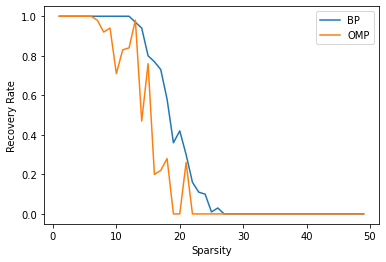
\includegraphics[scale = 0.7]{bp_omp_recovery_rate_m_constant_final.png}
    \caption{Recovery rate of random sparse vectors over a set of 100 Gaussian matrices, as a function of sparsity for fixed ($m=50,N=200$).}
    \label{rec_rate_spar}
\end{figure}

\begin{figure}
    \centering
    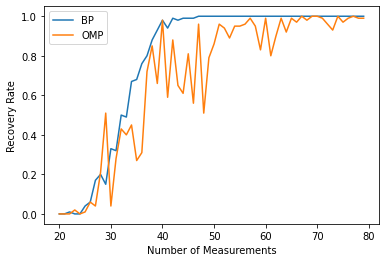
\includegraphics[scale = 0.7]{bp_omp_recovery_rate_s_constant.png}
    \caption{Recovery rate of random sparse vectors over a set of 100 Gaussian matrices, as a function of number of measurements for fixed ($s=10,N=200$).}
    \label{rec_rate_meas}
\end{figure}

These graphs, though noisy as a result of randomness and low sample size, demonstrate a few key components of compressed sensing, namely that after a certain point recovery is virtually guaranteed, whereas there is a quick drop-off to never being successful. In addition, orthogonal matching pursuit under-performs basis pursuit in both cases, though not to an incredibly large degree. In fact, the utility of orthogonal matching pursuit is that it is usually good enough, while being much faster to run than basis pursuit.

We note also that the higher jaggedness of Figure \ref{rec_rate_meas}, in comparison to Figure \ref{rec_rate_spar}, is likely due to the fact that we re-randomized the matrices at every value of $m$ for the former, whereas the matrices for the latter were randomized at the start but constant for every value of $s$. This does however support the notion that recovery success depends on the matrix to a good degree, as the more volatile graph was produced with more randomness in the matrices used.

In Figure \ref{bp_omp_time} we plot the average amount of time, per matrix, that basis pursuit and orthogonal matching pursuit took respectively to run, during the simulation where we varied $s$, which corresponds to Figure \ref{rec_rate_spar}. Notably, basis pursuit is clearly much more costly in terms of running time as compared with orthogonal matching pursuit. Nevertheless, the low sample size and low values of $N$ and $m$ are significant considerations, as compressed sensing as a method is geared for use on large data sets.

\begin{figure}
    \centering
    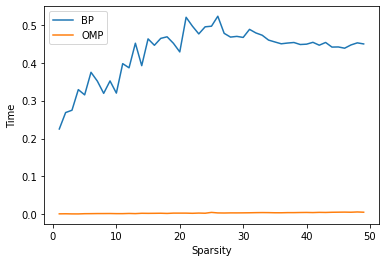
\includegraphics[scale = 0.7]{bp_omp_time_m_constant_final.png}
    \caption{The average amount of time it took to run basis pursuit and orthogonal matching pursuit on an individual matrix, for each value of $s$ from Figure \ref{rec_rate_spar}.}
    \label{bp_omp_time}
\end{figure}

In addition, as seen in Figure \ref{omp_time}, the main factor for the running time of orthogonal matching pursuit is the sparsity $s$, which makes sense as the algorithm computes $s$ iterations of its core steps. As such, when $s$ is varied, the graph of running time is about linear, meaning that as the data set size and thus $s$ increases, orthogonal matching pursuit will lose some of its advantages over basis pursuit, but the extent to which it was already faster will ensure that it remains the more efficient computation option.

\begin{figure}
    \centering
    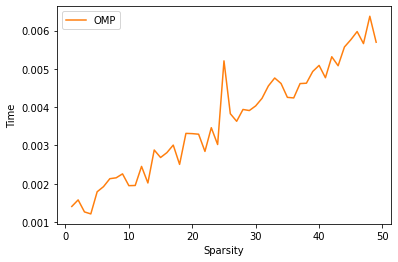
\includegraphics[scale = 0.7]{omp_time_m_constant_final.png}
    \caption{The average amount of time it took to run orthogonal matching pursuit on an individual matrix, for each value of $s$ from Figure \ref{rec_rate_spar}.}
    \label{omp_time}
\end{figure}

\subsection{A Simulated Comparison of Choices of Measurement Matrix}\label{sim-matrix}

We will also use a simulation of our compressed sensing algorithms to obtain a general understanding or at the very least a simple visualization of how the choice of measurement matrix $\bdA$ affects the performance of sparse recovery, in particular the recovery rate. In Section \ref{omp-bp-comparison} we saw the performance of basis pursuit using $\ell^2$-normalized Gaussian measurement matrices, so we will use this setting as a baseline against which to compare, which is an especially useful comparison since we have an idea from Theorem \ref{rip-gaussian} as to why Gaussian matrices are a good choice. The choice of basis pursuit for the common recovery algorithm also makes sense since it is theoretically the most successful algorithm, though it is slow.

We will simulate two comparisons: the first between Gaussian, Laplace, and Cauchy matrices, and the second between Gaussian and deterministic matrices. First we will discuss the first two of these distributions, and specifically why we include them in our discussion. The Laplace distribution is often known alternatively as the "double exponential" distribution, since its PDF (probability density function) is symmetric about the origin and has the shape of the exponential PDF on either side. As such, the Laplace distribution is an example of a subexponential distribution, which we discussed briefly in Section \ref{random-matrix}. The Cauchy distribution, meanwhile, is defined as the ratio of two independent standard Gaussian random variables. Unlike the Gaussian or Laplace, the Cauchy distribution has a much fatter tail that decays at a rate slower than exponential. The best way to think about this contrast of tails is that the subgaussian and the subexponential have light tails, with the subexponential being one degree heavier, while distributions with polynomial tails have much heavier tails. Figure \ref{density-plot} has an illustration of the differences between the Gaussian, Laplace, and Cauchy, in terms of the thickness of their tails.

\begin{figure}
    \centering
    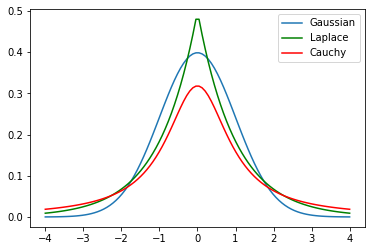
\includegraphics[scale = 0.7]{density_plot_final.png}
    \caption{Plots of the PDFs for the standard Gaussian, Laplace, and Cauchy distributions. Note that the relative sizes of the distribution tails are determined by how quickly the value of the function decreases as the argument tends towards $\pm\infty$.}
    \label{density-plot}
\end{figure}

The simulations for Laplace and Cauchy will be identical except for matrix distribution, using the same structure as the simulations from Figure \ref{rec_rate_meas}, namely of varying the number of measurements $m$, while keeping a fixed $s=10$ and $N=200$, and at every value of $m$ computing a new set of 100 random matrices. Both the Laplace and Cauchy matrices will be scaled by a factor of $\frac{1}{\sqrt{m}}$, the same factor by which the Gaussian matrix is scaled. We do this so that we can make a comparison between the performance of the matrices with a clear conscience. If we were to try to scale such that each matrix had $\ell^2$-normalized columns in expectation, then we would have to scale the Laplace matrix by $\frac{1}{\sqrt{2m}}$, since a standard Laplace variable has variance 2, and we would not be able to scale the Cauchy matrix to achieve this end, as the Cauchy distribution does not have a finite mean or variance. As such, we simply use the scaling factor from the Gaussian matrix to maintain some consistency.

\begin{figure}
    \centering
    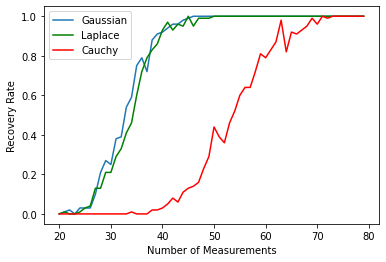
\includegraphics[scale = 0.7]{gaussian_laplace_cauchy.png}
    \caption{Recovery rate of random sparse vectors via basis pursuit for sets of 100 random Gaussian, Laplace, and Cauchy matrices, as a function of number of measurements for fixed $(s=10,N=200)$.}
    \label{laplace_cauchy_graph}
\end{figure}

Figure \ref{laplace_cauchy_graph} shows exactly how thin the margins between subgaussian and supexponential distributions can be. Despite the recovery result in Theorem \ref{rip-l1}, which specifies a subgaussian random measurement matrix setting, Laplace matrices provide an only slightly less successful recovery rate, at least in this isolated experiment, with small values of $s=10$ and $N=200$. This graph is an important reminder that the basic theoretical results such as Theorem \ref{rip-l1} are designed to deal with the worst-case scenario, and are often only necessary when the sample size is much larger than what our experiments use.

However, comparing the recovery rate with Gaussian random matrices versus Cauchy random matrices illustrates why exponentially-decaying tails are a necessity. In Figure \ref{laplace_cauchy_graph}, we see that while the Cauchy setting eventually reaches a good recovery rate, it requires a much higher number of measurements $m$, which presumably will scale poorly as the dimensionality increases.

We can also visualize via simulation why choosing a random measurement matrix is a much more successful setting than a general deterministic matrix. The following simulation involves choosing, for each $m$, one random Gaussian $m\times N$ matrix and the deterministic $m\times N$ matrix $\bdA(m,N)$ chosen according to the following rule:

\begin{align}\label{det-def}
    \bdA_{ij}=i+(j\mod(i+2)),
\end{align}

where $\bdA_{ij}$ is the entry in the $i$th row and $j$th column of $\bdA$, with $i\in[m]$ and $j\in[N]$. An example of this matrix, with shape $4\times 6$, is the following:

\begin{align*}
    \bdA(4,6)=
    \begin{pmatrix}
        0 & 1 & 0 & 1 & 0 & 1 \\
        1 & 2 & 3 & 1 & 2 & 3 \\
        2 & 3 & 4 & 5 & 2 & 3 \\
        3 & 4 & 5 & 6 & 7 & 3 \\
    \end{pmatrix}.
\end{align*}

This formula for the deterministic matrix was chosen to be a pre-determined formula while producing a matrix without many dependencies between columns or rows, though because $m<N$ the columns will of course be linearly dependent. This choice is in contrast to, say, choosing a matrix of all ones.

\begin{figure}
    \centering
    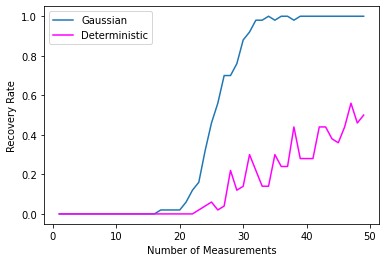
\includegraphics[scale = 0.7]{gaussian_det.png}
    \caption{Recovery rate via basis pursuit of a set of 50 $s$-sparse vectors, for a single random Guassian or deterministic matrix defined according to (\ref{det-def}), as a function of number of measurements for $(s=10,N=100)$.}
    \label{det-graph}
\end{figure}

Our simulation then takes fixed $s=10,N=100$, and produces the plot shown in Figure \ref{det-graph}. As for the Laplace and Cauchy matrices, we scale both the Gaussian and the deterministic matrix by a factor of $\frac{1}{\sqrt{m}}$ just so the comparison is valid. While the Gaussian setting experiences total success soon after $m=30$, the deterministic matrix is unable to exceed a success rate of 0.5. While we might expect this success rate to increase as $m$ continues to increase, it is clear that this particular choice of determinstic matrix is a very poor choice of measurement matrix, and will likely become much worse as the dimensionality of the problem increases.

After only investigating this single particular choice of deterministic matrix, we do not have enough evidence to generalize to the assertion that any deterministic matrix will fail, which is in fact not the case. In fact, the matrices we are technically deterministic, as they are only \textit{pseudorandom}, as computers do not have the capacity to produce truly random values. In addition, other formulations for deterministic measurement matrices which work well for sparse recovery are possible, including Fourier frames \cite{fou-rau}, which can be empirically shown to perform well for sparse recovery. However, the main barrier in this regard, which is a crucial part of ongoing research, is how to prove that such deterministic settings work \cite{fou-rau}. In any case, it is clear from Figure \ref{det-graph} that it is certainly possible to produce deterministic measurement matrices which are poorly suited for compressed sensing, despite efforts to construct them in a somewhat pseudorandom-looking way.

\section{Compressed Sensing in Application: MRI Technology}\label{app}

So far we have detailed the initial theory of compressed sensing, involving the conditions under which exact recovery succeeds and the algorithms which are often used to accomplish this task. However, the main utility of compressed sensing lies in its application, and there are many more complications to keep in mind when working with real-world data. Two particular considerations are stable and robust recovery, the former being a notion of success even when the vectors are not exactly sparse, and the latter being a notion of success even when taking into account measurement error \cite{fou-rau}.

As such, we aim in this section to detail a specific application of compressed sensing in order to better understand the challenges of applying the method. The application area in question is magnetic resonance imaging (MRI), which is most well known for its use in medical situations, including for imaging the brain or spine. The technology makes use of an external magnetic field to get certain protons to emit radio frequencies which can then be tracked and coalesced into images. In particular, these protons often come from water or fat molecules in the human body. For a more in-depth understanding of the physics behind MRI the interested reader may refer to \cite{wm}.

For our purposes the key takeaway is that traditionally MRI machines needed to take many samples in order to fully form the desired images, which was costly, both in terms of time spent and the physical cost of the equipment. Thus, the work of Lustig et al. in 2007, in the aftermath of the seminal compressed sensing literature, made the crucial step of taking advantage of the inherent sparse structure of MRI images to apply compressed sensing methods \cite{lustig}. We discuss the general mathematical definition of the MRI problem in Section \ref{mri-math} and overview the way in which one can harness the sparse structure of MRI in Section \ref{mri-cs-setting}. As of the time of writing, this advancement in MRI technology remains one of the most significant successes of compressed sensing and a signature example of its utility \cite{wm}.

\subsection{Mathematical Formulation of MRI}\label{mri-math}

The subsequent notation we introduce for interpreting the MRI image acquisition problem is adapted from Wright and Ma \cite{wm}.

While the exact means by which a "signal" is produced relies on the physics (and for a more detailed exposition in this regard we refer the reader to \cite{wm}), the ultimate product is a function in two variables $\bdM(x,y)$ which at a high level represents the magnetic field at coordinates $(x,y)$ for a specific third axis value $z_0$. In order to obtain a complete picture of the target, we produce a signal computed with the magnitude $|\bdM(x,y)|$ defined at time $t$ by 
\begin{align}
    s(t)=e^{-i\omega_0t}\int_x\int_y|\bdM(x,y)|e^{-i(k_x(t)x+k_y(t)y)}dxdy,
\end{align}
where $\omega_0$ is a set frequency known in the literature as the \textit{Larmor frequency}, and the functions $k_x,k_y$ form a transformation from $(x,y)$ to what is known as \textit{k-space}, based on the properties of the gradient of a second magnetic field \cite{wm}. Then re-expressing this function with regard to values $k_x,k_y$ and ignoring the $e^{-\omega_0t}$ term we get
\begin{align}
    S(k_x,k_y)=\int_x\int_y|\bdM(x,y)|e^{-i(k_xx+k_yy)}dxdy,
\end{align}
which is essentially the 2D Fourier transform of $|\bdM(x,y)|$ at $k_x,k_y$. For some intuition regarding the presence of a Fourier transform, note that the purpose of a Fourier transform is often to move between the spatial and frequency domain, and the MRI measurement process is better equipped to work in the frequency domain. In addition, note that this formulation motivates our insistence on giving compressed sensing results in complex dimensions (i.e. $\bdx\in\BC^N,\bdy\in\BC^m,\bdA\in\BC^{m\times N}$), since the function of complex Fourier transform values as measurements is a natural setting.

With this Fourier structure, it is then a natural goal to want to use an inverse Fourier transform to recover the image $I(x,y)$ (in the form of the function $|M(x,y)|$), with enough measurements at various frequencies $\{(k_x(t_i),k_y(t_i)\}_{i\in I}$ for some index set $I$ corresponding to different times $\{t_i\}_{i\in I}$. 

Recovering a continuous function however is difficult and unnecessary, since any image we produce will have some finite resolution. Thus, we treat $I(x,y)$ as a function on an $N\times N$ grid, and call $\bdu=(k_x,k_y)$ the vector of coordinates across the chosen times \cite{wm}, in which case our measurement will be of the form
\begin{align}\label{y-mri}
    \bdy(\bdu)=\mathcal{F}[I(x,y)](\bdu),
\end{align}
where $\mathcal{F}$ is the discrete Fourier transform, in the form of an $m\times m$ matrix $\mathcal{F}[I(x,y)]$ where $m=N^2$. Then the image at point $(x,y)$ is recovered via the inverse discrete Fourier transform at $\bdy(\bdu)$.

In is however redundant to recover these $I(x,y)$ values, of which there are $m$, so sampling the entire transform domain is not necessary. Meanwhile, traditional signal processing knowledge, from our discussion of Theorem \ref{n-s} (the Nyquist sampling rate), says that if our frequencies are bounded above by $f_{\max}$, then we only need to sample at a rate of over $2f_\max$ frequencies. Yet this rate can still be costly, as we discussed in the introduction, so based on the initial work by Lustig et al. \cite{lustig}, we look for a notion of sparsity with the goal of applying compressed sensing techniques.


\subsection{Translating MRI to a Compressed Sensing Setting}\label{mri-cs-setting}

The "sparsity" of MR images is a illuminating example of the power of sparse thinking, in that these images are certainly not sparse, given most of their pixels are nonzero, but they do have a well-defined structure, which leads to sparsity in a given basis. In particular, MR images (and many natural images), when viewed as functions in 2D space, are sparse in the wavelet transform domain \cite{lustig}, which is associated with a collection $\{\psi_i\}_{i\in[N^2]}$ of functions on 2D space \cite{wm}. We reserve a full explanation of the definition of wavelets and why images are sparse in the wavelet domain to the literature \cite{lustig}, but an intuitive picture to keep in mind is that most images of a certain type follow various patterns that allow them to be represented by a combination of smaller set pieces. 

To formalize the function of this wavelet basis, we think of $\Phi$ taking an image to a representation $\bdx$ in the wavelet domain: $\Phi[I]=\bdx$, with the natural inverse $\Psi=\Phi^{-1}$ sending the vector $\bdx$ of coefficients to a 2D image:
\begin{align*}
    I=\Psi[\bdx]=\sum_{i\in[N^2]}\bdx_i\psi_i.
\end{align*}
The notion of sparsity for this representation is that a small number of the coefficients $\bdx_i$ are nonzero. There are other alternatives to the wavelet basis \cite{wm}, but it is one of the clearer and more often used options, and as such we proceed to give a compressed sensing formulation which takes advantage of this newly found sparse representation.

Using this representation of $I$, we can express our measurement $\bdy$ in (\ref{y-mri}) as
\begin{align}\label{y-mri2}
    \bdy=\mathcal{F}[\Psi\bdx],
\end{align}
where $\bdz:=\Psi\bdx$ is a vector with shape $N^2$ representing $I$. Taking $m\ll N^2$ measurements we can produce a $m\times N^2$ Fourier matrix $\mathcal{F}_m\in\BC^{m\times N^2}$, so we can re-formulate (\ref{y-mri2}) as 
\begin{align*}
    \bdy=\mathcal{F}_m\Psi\bdx=\bdA\bdx
\end{align*}
where $\bdA:=\mathcal{F}_m\Psi$ is now a measurement matrix which completes the set of measurements necessary for compressed sensing. It turns out that when the $m$ measurements are sampled randomly from the full $N^2\times N^2$ Fourier matrix $\mathcal{F}$, the matrix $\bdA$ is sufficiently incoherent and then by our coherence-related recovery results in Section \ref{coh-section} our compressed sensing methods will work. However, due to the distribution of the wavelet coefficients a density-based sampling scheme, as opposed to a uniformly random one, is better to use \cite{wm}. Once a vector $\bdx^*$ is recovered via compressed sensing, the image is recovered by applying $\Psi:$ $\bdz^*=\Psi\bdx^*$.

As with any application area, feasibility concerns will arise and necessitate alterations to the ideal compressed sensing setting. A primary challenge for MRI involves the infeasibility of a fully random sampling scheme, namely that an MRI machine cannot sample at completely random locations, instead able to sample along trajectories in the $k$-space \cite{wm}. Thus a few common solutions include to sample a set of radii or a set of concentric circles from the center of the image. 

A further concern is measurement error, which is common in the MRI setting in the form of thermal noise, a natural outcome of the high-power technology utilized for the method. The subsequent minimization problem accounts for this possibility by bounding the $\ell^2$ measurement error by $\eta$:
\begin{align*}
    \text{minimize }\|\bdz\|_1 \ \ \text{subject to }\|\bdA\bdz-\bdy\|_2\leq\eta,
\end{align*}
which is equivalent to a notion of \textit{robust} recovery \cite{wm, fou-rau}. Robust recovery, while not discussed to a great extent in this paper, is a naturally important consideration for any application of compressed sensing due to the ubiquity of noise in real-world measurements.

\section{Conclusion and Next Steps for Compressed Sensing}

In this paper we have given a review of the early theory for compressed sensing, including the intuition for why the method works, the conditions under which sparse recovery is successful, and the main algorithms used in its implementation. We have also introduced an example of the application of compressed sensing to MRI technology. 

However, the theory presented is almost entirely preoccupied with the most ideal case, being of exact recovery for exactly sparse signals, two assumptions which are both unrealistic. These issues obtain consideration in the form of robust and stable recovery respectively, which were mentioned briefly in Section \ref{app}. These considerations are important since the main work currently going into compressed sensing is in formatting the theory for application. Now that the significance of sparsity and structure are well understood and the dust has settled on the initial flurry of seminal work during the mid to late 2000's, compressed sensing has its place as a pillar of practical signal processing.

Alongside MRI technology, which was one of the earliest applications of compressed sensing, and might be considered the most significant, the field has been applied to other areas of imaging, such as radar \cite{yang}. Additionally, a signature new technology born out of compressed sensing is the so-called single-pixel camera, which was built to take advantage of sparsity assumptions in order to make simpler measurements and as a result be much more efficient \cite{duarte}. Compressed sensing is also extensively used in the field of communications, in many different ways, making the field one of the more robust areas of application for compressed sensing \cite{choi}.

Due to the ubiquity of its core assumption of sparsity and in particular, structure, which is found in most natural phenomena, researchers have proposed compressed solutions to many additional problems, including facial recognition, video processing, and speech processing. Of course each new set of data provides its own challenge, a flavor for which we got through our discussion of MRI technology. However, there are a few common challenges that remain significant frontiers for the field.

Perhaps the most significant frontier to conquer is a general acquisition scheme for measurements \cite{rani}. As mentioned in Section \ref{random-matrix}, the most common setting for compressed sensing is with a random measurement matrix. Constructing deterministic matrices for which one can prove their optimality in the sparse recovery sense is still a difficult open problem \cite{fou-rau}. Since true randomness is hard to accomplish, especially given the limitations of many real-world technologies such as MRI machines, formulating a measurement scheme which achieves the requisite measurement matrix conditions, often through a pseudorandom process, is of the utmost importance. As per mathematician Robert Coveyou's famous titular adage: "random number generation is too important to be left to chance" \cite{coveyou}.

One potential alternative that has been in the works for about a decade is structured compressed sensing, which approaches the issue of constructing a suitable measurement matrix by taking a so-called "structured" matrix, which is produced by taking the matrix to be a basis which is orthonormal to the basis in which the signal is sparse \cite{fou-rau}. Among the many areas in which structured compressed sensing can be utilized is in image resolution. However, as with any method there are trade-offs, with structured compressed sensing being an overall simpler method with a faster measurement process, while needing more measurements and having a harder time satisfying the restricted isometry property \cite{rani}. As such some researchers are looking for ways to provide for sparse recovery while bypassing the restricted isometry property, which is usually the most common theoretical recovery guarantee.

As we saw with MRI, there are also many application-specific challenges that arise, including a necessity for new algorithms, a universal measurement process, and more efficient computation. These challenges just serve to keep compressed sensing, though certainly past its heyday of the late 2000's and early 2010's, an intriguing topic for mathematicians and engineers alike, with its rigorous mathematical theory and rich application power. In the modern world of big data, where efficient computation is at a premium, it is a field that we cannot afford to overlook.

\begin{appendices}

\section{Recovery Conditions for Basis Pursuit and Orthogonal Matching Pursuit}\label{bp-omp-conds}

In the first part we will develop the theory necessary to prove Theorems \ref{ric-bp} and \ref{coh-thm}, with respect to the success of basis pursuit, which as previously mentioned is the $\ell^1$-minimization (\ref{l1}). This theory is adapted from Foucart and Rauhut \cite{fou-rau}.

Before we introduce Theorem \ref{bp-cond} which will allow us to complete these proofs in Section \ref{theory}, we introduce a third notion of matrix niceness, alongside incoherence and the restricted isometry property, known as the null space property. Note that we present the null space property here and not in the main body since it is most useful as an intermediate step, whereas coherence and the restricted isometry constant are easier to work with.

\begin{Def}\label{nsp} A matrix $\bdA\in\BC^{m\times N}$ satisfies the \textit{null space property} relative to a set $S\subset[N]$ if
\begin{align}\label{nsp-prop}
    \|\bdv_S\|_1<\|\bdv_{\bar S}\|_1 \ \ \text{for all nonzero } \bdv\in\ker(\bdA).
\end{align}
\end{Def}

We obtain a subsequent reformulation of this property (\ref{nsp-prop}) by adding $\|\bdv_S\|_1$ to both sides of the inequality.

\begin{align}\label{nsp-ref}
    2\|\bdv_S\|_1<\|\bdv\|_1 \ \ \text{for all nonzero }\bdv\in\ker(\bdA).
\end{align}

We can also define the null space property \textit{of order} $s$, which holds for a matrix $\bdA$ if $\bdA$ satisfies the null space property relative to $S$ for all $\card(S)\leq s$. Then the natural connection of the null space property to $\ell^1$-minimization is given by the following theorem, which we also prove.

\begin{Th}\label{bp-cond} For a matrix $\bdA\in\BC^{m\times N}$, every $s$-sparse $\bdx\in\BC^N$ is uniquely recovered by basis pursuit with $\bdy=\bdA\bdx$ if and only if $\bdA$ satisfies the null space property of order $s$.

\end{Th}

\begin{proof}
    First we assume that basis pursuit uniquely recovers $\bdx$ with the given inputs, so any $s$-sparse $\bdx$ is the unique minimizer of $\|\bdz\|_1$ under the constraint that $\bdA\bdz=\bdA\bdx$. Thus, for any nonzero vector $\bdv\in\ker(\bdA)$, we can take any index set $S\subset[N]$ with $\card(S)\leq s$ and $\bdv_S$ will be an $s$-sparse vector meaning it is the unique minimizer of $\|\bdz\|_1$ under the constraint that $\bdA\bdz=\bdA\bdv_S$. However, $\bdA(\bdv_S+\bdv_{\bar S})=\bdA\bdv=\mathbf{0}$ and thus $\bdA(-\bdv_{\bar S})=\bdA\bdv_S$ where $-\bdv_{\bar S}\neq\bdv_S$ as $\bdv\neq\mathbf{0}$, so $\|\bdv_S\|_1<\|\bdv_{\bar S}\|_1$ since $\bdv_S$ is the unique minimizer.\\
    
    Next we assume that $\bdA$ satisfies the null space property of order $s$, so for any nonzero $\bdv\in\ker(\bdA)$ and index set $S\subset[N]$ with $\card(S)\leq s$, $\|\bdv_S\|_1<\|\bdv_{\bar S}\|_1$. Then taking $\bdx$ $s$-sparse, we will show that $\bdx$ is the unique minimizer of $\|\bdz\|_1$ with the constraint that $\bdA\bdz=\bdA\bdx$. For $\bdz\neq\bdx$ satisfying $\bdA\bdz=\bdA\bdx$, we can define the nonzero vector $\bdv:=\bdx-\bdz\in\ker(\bdA)$, which allows us to bound:
    \begin{align*}
        \|\bdx\|_1\leq\|\bdv_S\|_1+\|\bdz_S\|_1<\|\bdv_{\bar S}\|_1+\|\bdz_S\|_1=\|-\bdz_{\bar S}\|_1+\|\bdz_S\|_1=\|\bdz\|_1.
    \end{align*}
    This utilizes the fact that $\bdx$ is only supported on $S$ for the first inequality, and for the equality that $\bdv_{\bar S}=-\bdz_{\bar S}$.
\end{proof}

At this point we are done, with what was a fairly clean proof which provides us the tools necessary to prove the basis pursuit parts of Theorems \ref{ric-bp} and \ref{coh-thm}.

Next we will state and prove the proposition that allows us to prove the orthogonal matching pursuit portion of Theorem \ref{coh-thm}, the statement and proof of which are likewise adapted from Foucart and Rauhut \cite{fou-rau}.

\begin{Prop}\label{omp-cond} For a matrix $\bdA\in\BC^{m\times N}$, each nonzero $\bdx\in\BC^N$ supported on an index set $S\subset[N]$ with $\card(S)=s$ is recovered from input measurement vector $\bdy=\bdA\bdx$ after at most $s$ iterations of orthogonal matching pursuit if and only if $\bdA_S$ is injective and for all nonzero $\bdw=\bdA\bdz$ with $\supp(\bdz)\subset S$,
\begin{align}\label{omp-cond-ineq}
    \max_{j\in S}|(\bdA^*\bdw)_j|>\max_{k\notin S}|(\bdA^*\bdw)_k|.
\end{align}
\end{Prop}

Here $\bdA_S$ is the matrix $\bdA$ constrained to only the columns corresponding to the $s$ indices in the set $S$, and $\bda_i$ is the $i$th column of the matrix $\bdA$. Note that $(\bdA^*\bdw)_i=\langle\bdw,\bda_i\rangle$, the latter of which we used in our proof of Theorem \ref{coh-thm}. Next we will prove the above proposition.

\begin{proof}
    Assuming first that orthogonal matching pursuit recovers each nonzero $\bdx$ in the given way, we see that the matrix $\bdA_S$ is injective since any vectors supported on $S$ which have the same measurement vector must be the same (otherwise orthogonal matching pursuit might not output the correct vector). Then we also know that the first index chosen by orthogonal matching pusuit is in the target index set $S$, meaning $\max_{j\in S}|(\bdA^*\bdy)_j|>\max_{k\notin S}|(\bdA^*\bdy)_k|$, which will be true for any $\bdy=\bdA\bdx$ for $\bdx$ supported on $S$, so we are done with the forwards direction.\\
    
    Next we assume that $\bdA_S$ is injective and (\ref{omp-cond-ineq}) holds for all relevant $\bdw$. We need to show that in the context of the orthogonal matching pursuit notation given in Section \ref{omp}, $S^n\subset S$ for all $n\in[s]$ and thus $S^s=S$, at which point $\bdx^s=\bdx$ by the injectivity of $\bdA_S$, correctly recovering the unique $s$-sparse signal $\bdx$. The base case is $S^0=\varnothing\subset S$, so we proceed inductively, assuming $S^n\subset S$ for some $0\leq n\leq s-1$, meaning $\bdw^n:=\bdy-\bdA\bdx^n=\bdA\bdz$ for some $s$-sparse $\bdz$. Thus by (\ref{omp-cond-ineq}) the next index $j_{n+1}\in S$ meaning $S^{n+1}\subset S$, so we are done.
\end{proof}

\section{Inequalities Involving the Restricted Isometry Constant and Coherence}\label{coh-ric}

First we give an alternative definition of the restricted isometry constant, using the matrix norm \cite{fou-rau}.

\begin{Def}\label{ric-alt} The $s$th restricted isometry constant $\delta_s$ of a matrix $\bdA\in\BC^{m\times N}$ is
\begin{align*}
    \delta_s:=\max_{S\subset[N],\card(S)\leq s}\|\bdA_S^*\bdA_S-\Id\|_{2\rightarrow2}.
\end{align*}
\end{Def}

Here the $^*$ operator is the conjugate transpose, and the $\|\cdot\|_{2\rightarrow2}$ norm is the operator norm from $\ell^2$ to $\ell^2$ defined as the maximum singular value of that matrix. The measure here intuitively gives the worst case scenario, under index sets $S$ with $\card(S)\leq s$, of how close $\bdA_S$, the restriction of $\bdA$ to the index set $S$, is to an isometry. With this definition we may then prove the following proposition relating the restricted isometry constant to coherence.

\begin{Prop}\label{ric-coh} If a matrix $\bdA\in\BC^{m\times N}$ has $\ell^2$-normalized columns, then its coherence and restricted isometry constants satisfy
\begin{align*}
\delta_1=0,\ \ \delta_2=\mu,\ \ \delta_s\leq\mu_1(s-1)=(s-1)\mu, \ \ s\geq2.
\end{align*}
\end{Prop}

To do this first we must understand the meaning of $\mu$, which is a more general notion of coherence, not associated with a sparsity $s$: $\mu:=\max_{1\leq i\neq j\leq N}|\langle\bda_i,\bda_j\rangle|$ is the coherence of $A$, where $\bda_i$ are the columns of $\bdA$. Now we will prove the first two parts Proposition \ref{ric-coh}, and cite a result for the third.

\begin{proof}
    First, the only index sets of size 1 are $S=\{j\}$, so for any such $S$, $\bdA_S^*\bdA_S=\bda_j^*\bda_j=\|\bda_j\|_2=1$, since the columns $\bda_j$ are normalized. The 1-dimensional identity matrix is just 1, so $\delta_1=0$.
    
    For $\delta_2$, we need to compute $\bdA_{\{i,j\}}^*\bdA_{\{i,j\}}$ for any $i\neq j$ with $\{i,j\}\subset[N]$, which will be $$\bdA_{\{i,j\}}^*\bdA_{\{i,j\}}=\begin{pmatrix}1 & \langle \bda_j,\bda_i\rangle \\ \langle \bda_i,\bda_j\rangle & 1\end{pmatrix}\Rightarrow\bdA_{\{i,j\}}^*\bdA_{\{i,j\}}-\Id=\begin{pmatrix}0 & \langle \bda_j,\bda_i\rangle \\ \langle \bda_i,\bda_j\rangle & 0\end{pmatrix}.$$ The eigenvalues of this matrix are $\pm|\langle\bda_i,\bda_j\rangle|$, so $\|\bdA_{\{i,j\}}^*\bdA_{\{i,j\}}-\Id\|_{2\rightarrow2}=|\langle\bda_i,\bda_j\rangle|$ and thus $$\delta_2=\max_{i\neq j}|\langle\bda_i,\bda_j\rangle|=\mu$$ as already defined. The $s\geq2$ case can be shown using Theorem 5.3 from \cite{fou-rau}, though I have the space to include neither it nor the proof thereof.
\end{proof}

Proposition \ref{ric-coh}, along the fact that the restricted isometry constant is non-decreasing in $s$, gives us the result (\ref{mu-relation}), since substituting $s+1$ for $s$ (where $s\geq1$), we have that $\delta_{s+1}\leq\mu_1(s)=s\mu$, where $\mu=\delta_2\leq\delta_{s+1}$.

\section{Basis Pursuit via Linear Programming}\label{lin-prog}

Linear programming is a fairly standard part of optimization literature, having a dedicated function (scipy.optimize.linprog) within the SciPy library in Python, which is what we used to implement basis pursuit in Section \ref{omp-bp-comparison}. A classic linear programming formulation, which is the one employed in the SciPy documentation is as follows:

\begin{align}\label{lp}
    \argmin_\bdx \bdc^\top\bdx \ \ \text{such that }\bdA_{ub}\bdx\leq b_{ub},\bdA_{eq}\bdx=\bdb_{eq},\bdl\leq\bdx\leq\bdu,
\end{align}

where $\bdc,\bdl,\bdu$ are all vectors of the same shape as $\bdx$, $\bdA_{ub},\bdA_{eq}$ are matrices, possibly of different shapes, and $\bdb_{ub},\bdb_{eq}$ are vectors of corresponding shapes to work with the matrix multiplication. An interpretation of the problem is to minimize some weighted version of $\bdx$ (which is distinct from the interpretation from the compressed sensing literature), subject to various linear constraints regarding $\bdx$, which form a feasible set in the form of a convex polytope. The standard formulation often omits the equality constraint, since it can be achieved through a re-formulation of the inequality \cite{chvatal}, but the SciPy formulation is easier to use. Solving this problem (\ref{lp}) is actually relatively straightforward to code, a more detailed explanation of which can be found in \cite{chvatal}.

In this appendix we restrict ourselves to simply showing how to formulate $\ell^1$-minimization (\ref{l1}), or basis pursuit, using linear programming. In particular, because basis pursuit minimizes $\|\bdz\|_1$, which is a sum of absolute entries, we need to produce a new formulation that does not use any absolute values. Thus, in addition to $\bdz$ we consider the vector $\bdt$, which we interpret as the absolute upper bound of $\bdz$, i.e. $|\bdz_i|\leq \bdt_i$ for all $i\in[N]$. Thus, what we actually want to minimize is $\sum_i\bdt_i$, subject to $\bdA\bdz=\bdy=\bdA\bdx$ as the equality constraint, and with $\bdz_i\leq\bdt_i,\bdz\geq-\bdt_i$ for all $i$, or in other words $I_N\bdz-I_N\bdt\leq\mathbf{0}$ and $-I_N\bdz-I_N\bdt\leq\mathbf{0}$.

To use all of these constraints we need to combine $\bdz$ and $\bdt$ into one vector $\bdw=(\bdz_1,...,\bdz_N,\bdt_1,...,\bdt_N)^\top$. Thus, our linear program takes the following inputs:

\begin{align*}
    \bdc=(0,...,0,1,...,1)^\top,\bdA_{eq}=\begin{pmatrix}\bdA \\ \mathbf{0}\end{pmatrix},\bdb_{eq}=\begin{pmatrix}\bdy \\ \mathbf{0}\end{pmatrix},\bdA_{ub}=\begin{pmatrix}I_N & -I_N \\ -I_N & -I_N\end{pmatrix},\bdb_{ub}=\mathbf{0}.
\end{align*}

They have respective shape $2N\times 1$ for the $\bdc$ of $N$ zeroes and $N$ ones, $2m\times N$ for $\bdA_{eq}$, $2m\times 1$ for $\bdb_{eq}$, $2N\times 2N$ for $\bdA_{ub}$, and $2N\times 1$ for $\bdb_{ub}$.  No $\bdl,\bdu$ values are required as the constraints of basis pursuit were already implement by the previous constraints.

\end{appendices}

\begin{thebibliography}{99} 

\bibitem{agresti} Agresti, A. (2015). Foundations of Linear and Generalized Linear Models. Hoboken, NJ: Wiley. 

\bibitem{candes} Cand\`{e}s, E.J., Romberg, J., Tao, T. (2006). Robust uncertainty principles: exact signal reconstruction from highly incomplete frequency information. IEEE Transactions on Information Theory, 52(2), 489-509.

\bibitem{choi} Choi, J.W., Shim, B., Ding, Y., Rao, B., Kim, D.I. (2017). IEEE Communications Surveys Tutorials, 19(3), 1527-1550.

\bibitem{chvatal} Chv\'{a}tal, V. (1983). Linear Programming. New York, NY: W.H. Freeman and Company.

\bibitem{coveyou} Coveyou, R.R. (1969). Random number generation is too important to be left to chance. Studies in Applied Mathematics, 3, 70-111.

\bibitem{donoho} Donoho, D.L. (2006). Compressed sensing. IEEE Transactions on Information Theory, 52(4), 1289-1306.

\bibitem{duarte} Duarte, M.F., Davenport, M.A., Takhar, D., Laska, J.N., Sun, T., Kelly, K.F., Baraniuk, R.G. (2008). IEEE Signal Processing Magazine, 25(2), 83-91.

\bibitem{fou-rau} Foucart, S., Rauhut, H. (2013). A Mathematical Introduction to Compressive Sensing. New York, NY: Birkh{\"a}user. 

\bibitem{haz-maz} Hazimeh, H., Mazumder, R., Saab, A. (2020). Sparse Regression at Scale: Branch-and-Bound rooted in First-Order Optimization. arXiv pre-print. http://arxiv.org/abs/2004.06152.

\bibitem{kunis-rauhut} Kunis, S., Rauhut, H. (2008). Random Sampling of Sparse Trigonometric Polynomials, II. Orthogonal Matching Pursuit versus Basis Pursuit. Foundations of Computational Mathematics, 8(6), 737-763.

\bibitem{logan} Logan, B. (1965). Properties of high-pass signals. P.h.D. dissertation, Columbia University.

\bibitem{lustig} Lustig, M., Donoho, D., Pauly, J.M. (2007). Sparse MRI: The Application of Compressed Sensing for Rapid MR Imaging. Magnetic Resonance in Medicine, 58(6), 1182-1195.

\bibitem{narayanan} Narayanan, S., Sahoo, S. K., Makur, A. (2015). Greedy Pursuits Assisted Basis Bursuit for Compressive Sensing. 2015 23rd European Signal Processing Conference, 694-698.

\bibitem{park-lee} Park, S., Lee, H. (2011). On the Derivation of RIP for Fandom Gaussian Matrices and Binary Sparse Signals. 2011 International Conference on ICT Convergence, 120-124.

\bibitem{rani} Rani, M., Dhok, S.B., Deshmukh, R.B. (2018). A Systematic Review of Compressive Sensing: Concepts, Implementations and Applications. IEEE Access, 6, 4875-4894.

\bibitem{tropp-gilbert} Tropp, J. A., Gilbert, A. C. (2007). Signal Recovery From Random Measurements Via Orthogonal Matching Pursuit. IEEE Transactions on Information Theory, 53(12), 4655-4666.

\bibitem{vershynin} Vershynin, R. (2015). "Estimation in High Dimensions: A Geometric Perspective", Sampling Theory, a Renaissance: Compressive Sensing and Other Developments. Springer International Publishing, 3-66.

\bibitem{wang} Wang, X. (2005). Volumes of Generalized Unit Balls. Mathematics Magazine, 78(5), 390-395.

\bibitem{wm} Wright, J., Ma, Y. (2021). High-Dimensional Data Analysis with Low-Dimensional Models: Principles, Computation, and Applications. Cambridge University Press.

\bibitem{yang} Yang, J., Jin, T., Xiao, C., Huang, X. (2019). Sensors, 19(14), 3100.

\end{thebibliography}



\end{document}
